\documentclass[%
    corpo=11pt,
    twoside,
    stile=classica,
    oldstyle,
    tipotesi=custom,
    greek,
    evenboxes,
]{toptesi}
%%%%%%%%%%%%%%%%%%%%%%%%%%%%%%%%%%%%%%%%%%%%%%%%%%%%

\usepackage[utf8]{inputenc}
\usepackage[T1]{fontenc}
\usepackage{lmodern}

\usepackage{hyperref}
\hypersetup{%
    pdfpagemode={UseOutlines},
    bookmarksopen,
    pdfstartview={FitH},
    colorlinks,
    linkcolor={blue},
    citecolor={blue},
    urlcolor={blue}
}

%%%%%%% use PDFLATEX 

\usepackage{lipsum} %to insert random text

\usepackage{geometry} %for the margins
\newcommand\fillin[1][4cm]{\makebox[#1]{\dotfill}} %for the dotted line in the frontispiece

\usepackage{dcolumn}
\newcolumntype{d}{D{.}{.}{-1} } %to vertical align numbers in tables, along the decimal dot

\usepackage{amsmath}
\usepackage{amssymb}

\usepackage{natbib} % for the bibliography
\bibliographystyle{plainnat}

%%%%%%% Local definitions
\newtheorem{osservazione}{Osservazione}% Standard LaTeX
\newtheorem{observation}{Observation}% Standard LaTeX

%%%%%%%%%%%%%%%%%%%%%%%%%%%%%%%%%%%%%%%%%%%%%%%%
%%%%%%%%%%%%%%%%%%%%%%%%%%%%%%%%%%%%%%%%%%%%%%%%

\begin{document}\errorcontextlines=9

\begin{titlepage}
\newgeometry{left=1cm,right=1cm,top=3cm,bottom=3.5cm}  %specific margins for this page

\begin{center}

{\huge POLITECNICO DI TORINO}\\[1.5cm]
\textbf{Corso di Laurea Magistrale in Ingegneria Informatica}\\[0.5cm]
\textit{Orientamento Artificial Intelligence and Data Analytics}\\[3cm]


{\Large Tesi di Laurea Magistrale}\\[0.5cm]
\textbf{\LARGE Dai pixel ai portafogli finanziari: generare scenari di mercato realistici tramite variational autoencoder }\\[2cm]

\includegraphics[width=0.2\textwidth]{./Pictures/logo_polito_2021.jpg}
\vspace{4cm}


\begin{minipage}{0.85\textwidth}
\begin{flushleft}\large
\textbf{Relatori} \hfill \textbf{Candidato}\\
prof. Flavio Giobergia \hfill Dylan Magliano\\
prof. Sergio Caprioli \hfill Matricola s337915\\
\textit{firma dei relatori} \hfill \textit{firma del candidato}\\[0.35cm]
\fillin\ \hfill \\
\fillin\ \hfill \fillin
\end{flushleft}
\end{minipage}

\vfill

Anno Accademico 2025-2026
\end{center}

\restoregeometry %restor default margins 

\end{titlepage} %the frontispiece

%%%%%%% Dedication
\ifclassica%
\begin{dedica}
    A mio padre\\
    \vspace{1em}
    \textdagger\ A mio nonno Pino
\end{dedica}
\fi
%%%%%%% 

\sommario%summary
Il presente lavoro di tesi si inserisce nel contesto della finanza quantitativa e del \emph{risk management}, affrontando le limitazioni dei modelli deterministici nella stima delle matrici di correlazione empiriche, tipicamente affette da rumore statistico e limiti di campionamento storico. Si propone un framework basato sul \emph{deep learning} per la compressione, ricostruzione e generazione stocastica di scenari di mercato realistici.

La metodologia si basa sull'analisi dei rendimenti giornalieri di un campione rappresentativo di 100 titoli dell'indice S\&P 500 nell'orizzonte temporale 2000-2020, selezionati per preservare l'eterogeneità settoriale del mercato. A partire dalle matrici di correlazione empiriche opportunamente pre-processate, viene condotto uno studio comparativo sistematico tra Principal Component Analysis (PCA), Autoencoder Lineari (Linear AE), Autoencoder Profondi non lineari (AE) e Variational Autoencoder (VAE). Ciascun modello viene valutato sia sotto il profilo quantitativo --- attraverso metriche di errore quali \emph{Mean Squared Error} (MSE), \emph{Mean Absolute Error} (MAE), la norma di Frobenius e l'analisi comparativa del \emph{Minimum Spanning Tree} (MST) generato --- sia sotto il profilo qualitativo mediante algoritmi di \emph{clustering} gerarchico per verificare la conservazione delle aggregazioni settoriali naturali del mercato. I risultati empirici evidenziano come, nel dominio della pura ricostruzione storica, gli approcci lineari offrano prestazioni dominanti a causa della natura intrinseca del dataset finanziario.

Per superare i limiti dei modelli deterministici e abilitare la generazione stocastica, il VAE viene impiegato per campionare nuove matrici di correlazione sintetiche dallo spazio latente regolarizzato. Queste nuove configurazioni vengono sottoposte al medesimo protocollo di validazione qualitativa e quantitativa, oltre a una verifica rigorosa rispetto a cinque \emph{stylized facts} fondamentali: distribuzione asimmetrica verso valori positivi delle correlazioni \emph{pairwise}, aderenza dello spettro degli autovalori alla distribuzione di Marchenko-Pastur, validità della proprietà di Perron-Frobenius, conservazione della struttura gerarchica e topologia \emph{scale-free} dell'MST. Il confronto con matrici casuali tramite la \emph{Random Matrix Theory} (RMT) conferma la capacità del VAE di preservare tali proprietà strutturali dei mercati reali.

Infine, le matrici sintetiche generate e validate vengono impiegate all'interno di un motore di simulazione Monte Carlo per la stima del Value at Risk (VaR) e dell'Expected Shortfall (ES) su portafogli reali. L'architettura proposta dimostra come l'intersezione tra modelli generativi profondi e stilizzazioni empiriche consenta di catturare i rischi di coda in modo significativamente più robusto rispetto ai metodi storici convenzionali.

%%%%%%%%%%%%%%%%%%%%%%%%%%%%%%%%%%%%%%%%%%%%%%%%
%%%%%%%%%%%%%%%%%%%%%%%%%%%%%%%%%%%%%%%%%%%%%%%%

% \ringraziamenti%acknowledgements
% (Lasciato vuoto per futuri ringraziamenti)

%%%%%%%%%%%%%%%%%%%%%%%%%%%%%%%%%%%%%%%%%%%%%%%%
%%%%%%%%%%%%%%%%%%%%%%%%%%%%%%%%%%%%%%%%%%%%%%%%

%\tablespagetrue\figurespagetrue%to include the list of tables and figures - uncomment when you have at least one figure and table

\indici%table of content (automatically generated)

%%%%%%%%%%%%%%%%%%%%%%%%%%%%%%%%%%%%%%%%%%%%%%%%
%%%%%%%%%%%%%%%%%%%%%%%%%%%%%%%%%%%%%%%%%%%%%%%%

\mainmatter

% ==========================================================
% PARTE I: FONDAMENTI TEORICI
% ==========================================================
\part{Fondamenti Teorici}

\chapter{Introduzione}
\label{ch:introduzione}

\section{Contesto generale sull'asset allocation e la gestione del rischio}

L'ottimizzazione del portafoglio e la gestione del rischio rappresentano due dei pilastri fondamentali della finanza quantitativa moderna. A partire dal lavoro pionieristico di Harry Markowitz del 1952 sulla \emph{Modern Portfolio Theory} (MPT), il problema dell'allocazione ottimale delle risorse è stato formalizzato come un problema di ottimizzazione vincolata a due obiettivi contrapposti: la massimizzazione del rendimento atteso e la contestuale minimizzazione della varianza del portafoglio. In questo paradigma economico, la matrice di covarianza e, in modo equivalente, la matrice di correlazione tra i rendimenti delle diverse attività finanziarie giocano un ruolo matematico centrale, agendo come l'operatore lineare che quantifica il rischio sistematico e i benefici della diversificazione.

Parallelamente, l'evoluzione dei mercati globali e l'introduzione di framework normativi sempre più stringenti hanno spinto l'industria finanziaria verso l'adozione di metriche di rischio più sofisticate della semplice varianza. Tra queste, il \emph{Value at Risk} (VaR) e l'\emph{Expected Shortfall} (ES) sono diventati gli standard \emph{de facto} per la quantificazione delle perdite potenziali in condizioni di mercato avverse entro un determinato orizzonte temporale e livello di confidenza. 

La stima accurata di tali metriche di rischio di coda si affida ampiamente a metodologie di simulazione, tra cui spiccano le simulazioni Monte Carlo. L'efficacia e l'affidabilità di questi motori di simulazione dipendono in maniera critica dalla qualità e dal realismo degli scenari di mercato generati. Se i modelli matematici sottostanti non riescono a catturare fedelmente le interdipendenze e la struttura correlativa degli asset finanziari, le stime del rischio risultano inevitabilmente distorte, conducendo a decisioni di \emph{asset allocation} sub-ottimali e a una potenziale sottostima delle minacce sistemiche.

\section{Definizione del problema di ricerca e motivazione dell'uso dei modelli generativi profondi}

Il principale ostacolo nell'applicazione pratica dei modelli classici risiede nella natura intrinseca delle matrici di correlazione empiriche. Quando stimata a partire da serie storiche campionarie di rendimenti, la matrice di correlazione soffre in modo significativo del problema del rumore statistico e della non-stazionarietà dei mercati. Quando il numero di asset analizzati ($N$) è dello stesso ordine di grandezza della lunghezza della serie storica ($T$), la matrice empirica diventa instabile, introducendo autovalori spuri che degradano le performance degli algoritmi di ottimizzazione, un fenomeno ampiamente studiato nell'ambito della \emph{Random Matrix Theory} (RMT).

Nel presente lavoro, l'analisi si concentra sui rendimenti giornalieri dei titoli componenti l'indice S\&P 500 estratti lungo un ampio orizzonte temporale ventennale, compreso tra il 2000 e il 2020. Per mitigare la complessità computazionale e l'instabilità numerica associate alla dimensionalità dell'intero indice, mantenendo al contempo una fedele rappresentazione macroeconomica, la ricerca isola un paniere target di 100 asset. Al fine di evitare distorsioni e preservare la struttura intrinseca del mercato, la selezione viene eseguita tramite un algoritmo di campionamento stratificato, il quale garantisce il rispetto delle percentuali originali dei settori definiti dal \emph{Global Industry Classification Standard} (GICS).

I metodi tradizionali per gestire il rumore in tali matrici (come lo \emph{shrinkage} o il \emph{bootstrapping} storico) presentano forti limiti: tendono a linearizzare le relazioni eliminando anomalie informative o rimangono vincolati alla limitatezza storica, impedendo l'esplorazione di scenari estremi mai osservati precedentemente ma statisticamente plausibili. In questo panorama, i modelli generativi profondi (\emph{Deep Generative Models}) offrono un cambio di paradigma radicale. Architetture basate sui \emph{Variational Autoencoders} (VAE) consentono di mappare lo spazio ad alta dimensionalità delle matrici di correlazione empiriche in uno spazio latente continuo e regolarizzato. 

Per ottimizzare l'efficienza computazionale ed eliminare le ridondanze geometriche dovute alla simmetria intrinseca e alla diagonale unitaria, l'input dei modelli viene ridotto alla sola componente triangolare inferiore linearizzata delle matrici estratte dal sottoinsieme stratificato. Attraverso questo vincolo rappresentazionale, i modelli apprendono a comprimere e successivamente riprodurre l'intera struttura informativa. 

Al fine di mappare con rigore scientifico le capacità di questi strumenti, il framework introduce un doppio binario di validazione, sia qualitativo che quantitativo, applicato uniformemente a tutte le tecniche testate --- Principal Component Analysis (PCA), Autoencoder Lineari (Linear AE), Autoencoder Profondi (AE) e Variational Autoencoder (VAE) --- sia in fase di ricostruzione storica che, nel caso del VAE, in fase di generazione stocastica di nuove matrici campionate dallo spazio latente. L'integrazione di metriche di errore matematico classiche combinate con metriche topologiche finanziarie permette di valutare non solo l'accuratezza puntuale dei modelli, ma anche la conservazione delle proprietà strutturali profonde del mercato.

\section{Obiettivi della tesi}

Il presente lavoro di tesi si propone di progettare, implementare e validare un framework basato su architetture neurali profonde per la compressione, ricostruzione e generazione stocastica di matrici di correlazione finanziaria realistiche, finalizzato al miglioramento delle simulazioni di rischio.

Gli obiettivi specifici della ricerca possono essere declinati nei seguenti punti:
\begin{enumerate}
    \item \textbf{Sviluppo della pipeline di pre-processing e campionamento:} Definire una procedura rigorosa per l'estrazione e la pulizia dei rendimenti dei titoli dell'S\&P 500 (2000-2020), implementando il campionamento stratificato basato sui settori GICS per isolare i 100 asset di studio ed effettuando la scomposizione per estrarre le sole matrici triangolari inferiori come input ottimizzato.
    \item \textbf{Studio comparativo e validazione multidimensionale:} Analizzare ed evidenziare quantitativamente le performance strutturali di PCA, Linear AE, AE e VAE nella fase di ricostruzione storica, calcolando e confrontando sistematicamente metriche matematiche di errore rigide quali il \emph{Mean Squared Error} (MSE), il \emph{Mean Absolute Error} (MAE) e la norma di Frobenius. Tale impianto quantitativo viene integrato da una valutazione qualitativa e topologica --- applicata sia alle ricostruzioni storiche sia alle nuove matrici sintetizzate dal VAE --- mediante algoritmi di \emph{clustering} gerarchico per mappare visivamente la preservazione dei cluster settoriali e l'estrazione del \emph{Minimum Spanning Tree} (MST) per misurare la fedeltà della connettività strutturale degli asset.
    \item \textbf{Generazione stocastica e validazione tramite Stylized Facts:} Configurare l'impianto probabilistico del VAE per sintetizzare nuove matrici di correlazione tramite campionamento dello spazio latente, estendendo ad esse l'intero protocollo qualitativo/quantitativo e validandole rigorosamente rispetto ai cinque \emph{stylized facts} fondamentali del mercato rispetto alla \emph{Random Matrix Theory} (RMT).
    \item \textbf{Integrazione e stima del rischio:} Applicare le matrici sintetiche generate e validate dal VAE all'interno di scenari Monte Carlo per calcolare il Value at Risk e l'Expected Shortfall di portafogli reali, dimostrando l'efficacia del framework nel catturare i rischi di coda in modo più robusto rispetto ai metodi storici convenzionali.
\end{enumerate}
\chapter{Matrici di Correlazione in Ambito Finanziario}
\label{ch:matrici_finanziarie}

\section{Ruolo della correlazione nella Modern Portfolio Theory (Markowitz)}
\label{sec:markowitz}

La formalizzazione moderna del concetto di diversificazione trova il suo fondamento matematico nella \emph{Modern Portfolio Theory} (MPT) introdotta da Harry Markowitz nel 1952. Il paradigma fondamentale della MPT si basa sull'ipotesi che un investitore razionale selezioni le proprie strategie di allocazione considerando esclusivamente due parametri statistici: il rendimento atteso, inteso come misura del guadagno potenziale, e la varianza (o deviazione standard) dei rendimenti, assunta come metrica del rischio complessivo del portafoglio.

Si consideri un universo investibile composto da $N$ attività finanziarie rischiose. Sia $\mathbf{r} = [r_1, r_2, \dots, r_N]^T \in \mathbb{R}^N$ il vettore aleatorio dei rendimenti dei singoli asset, con vettore dei valori attesi $\mathbb{E}[\mathbf{r}] = \boldsymbol{\mu} \in \mathbb{R}^N$. Un portafoglio è univocamente definito dal vettore dei pesi $\mathbf{w} = [w_1, w_2, \dots, w_N]^T \in \mathbb{R}^N$, dove ciascuna componente $w_i$ rappresenta la frazione di capitale allocata nell'asset $i$-esimo, sotto il vincolo di piena allocazione delle risorse $\sum_{i=1}^N w_i = \mathbf{w}^T \mathbf{1} = 1$.

Il rendimento atteso del portafoglio, $E(R_p)$, è una combinazione lineare dei rendimenti attesi dei singoli titoli:
\begin{equation}
E(R_p) = \mathbb{E}[\mathbf{w}^T \mathbf{r}] = \mathbf{w}^T \boldsymbol{\mu}
\end{equation}

Il rischio del portafoglio, espresso mediante la sua varianza $\sigma_p^2$, è invece governato da una forma quadratica definita a partire dalla matrice di covarianza $\mathbf{\Sigma} \in \mathbb{R}^{N \times N}$:
\begin{equation}
\sigma_p^2 = \text{Var}(\mathbf{w}^T \mathbf{r}) = \mathbf{w}^T \mathbf{\Sigma} \mathbf{w} = \sum_{i=1}^N \sum_{j=1}^N w_i w_j \sigma_{ij}
\end{equation}
dove $\sigma_{ij}$ rappresenta la covarianza tra i rendimenti dell'asset $i$ e dell'asset $j$. La matrice di covarianza può essere fattorizzata isolando le componenti di volatilità individuale dalla struttura di interdipendenza lineare. Sia $\mathbf{D} \in \mathbb{R}^{N \times N}$ la matrice diagonale contenente le deviazioni standard dei singoli asset, $\mathbf{D} = \text{diag}(\sigma_1, \sigma_2, \dots, \sigma_N)$. La relazione fondamentale che lega la covarianza alla matrice di correlazione lineare di Pearson $\mathbf{C} \in \mathbb{R}^{N \times N}$ è espressa da:
\begin{equation}
\label{eq:sigma_decomposition}
\mathbf{\Sigma} = \mathbf{D} \mathbf{C} \mathbf{D}
\end{equation}

In virtù della decomponevolezza espressa nella \eqref{eq:sigma_decomposition}, l'elemento generico $C_{ij}$ della matrice di correlazione corrisponde al coefficiente di correlazione strutturale $\rho_{ij} = \frac{\sigma_{ij}}{\sigma_i \sigma_j}$, vincolato geometricamente nell'intervallo $[-1, 1]$. 

Il principio della diversificazione risiede interamente nelle proprietà algebriche di $\mathbf{C}$. Qualora i titoli presentino una correlazione lineare perfetta e positiva ($\rho_{ij} = 1 \, \forall i,j$), il rischio di portafoglio si riduce a una semplice media ponderata delle volatilità individuali, annullando qualsiasi effetto di mitigazione del rischio. Al contrario, la presenza di coefficienti $\rho_{ij} < 1$ garantisce che la deviazione standard del portafoglio sia strettamente inferiore alla combinazione lineare delle deviazioni standard dei singoli titoli. 

Nell'ambito dell'ottimizzazione di portafoglio secondo il criterio media-varianza, l'obiettivo si traduce nella determinazione della frontiera efficiente tramite la risoluzione di problemi di programmazione quadratica del tipo:
\begin{equation}
\min_{\mathbf{w}} \frac{1}{2} \mathbf{w}^T \mathbf{\Sigma} \mathbf{w} \quad \text{s.t.} \quad \mathbf{w}^T \mathbf{1} = 1, \quad \mathbf{w}^T \boldsymbol{\mu} = \mu_{\text{target}}
\end{equation}

In questo contesto, la matrice di correlazione opera come il nucleo geometrico che modella lo spazio delle soluzioni ammissibili. Errori di stima anche marginali nella struttura di $\mathbf{C}$ alterano drasticamente gli autovettori associati, distorcendo l'identificazione delle direzioni a varianza minima e conducendo a soluzioni di allocazione altamente instabili e inefficienti fuori campionario.

\section{Il problema del rumore nelle matrici empiriche}
\label{sec:rumore_empirico}

Nella pratica finanziaria, la vera matrice di correlazione della popolazione non è osservabile direttamente. Di conseguenza, gli analisti si affidano allo stimatore campionario standard, partendo dai log-rendimenti storici degli asset. Data una serie storica di rendimenti per $N$ attività finanziarie lungo un orizzonte temporale di $T$ giorni, si definisce innanzitutto la matrice di covarianza empirica $\hat{\mathbf{\Sigma}}$, il cui elemento generico è calcolato come:
\begin{equation}
\hat{\Sigma}_{ij} = \frac{1}{T-1} \sum_{t=1}^T (r_{i,t} - \bar{r}_i)(r_{j,t} - \bar{r}_j)
\end{equation}
dove $\bar{r}_i$ rappresenta la media campionaria del log-rendimento dell'asset $i$. 

La matrice di correlazione empirica $\hat{\mathbf{C}}$ viene quindi derivata normalizzando le covarianze per il prodotto delle rispettive deviazioni standard campionarie $\hat{\sigma}$:
\begin{equation}
\hat{C}_{ij} = \frac{\hat{\Sigma}_{ij}}{\hat{\sigma}_i \hat{\sigma}_j}
\end{equation}

Questo approccio incontra un limite strutturale severo, noto in letteratura come la ``maledizione della dimensionalità'' o problema del rumore statistico. L'accuratezza dello stimatore campionario dipende in modo critico dal parametro di spettro $q$, definito come il rapporto tra la dimensione spaziale e quella temporale del dataset:
\begin{equation}
q = \frac{N}{T}
\end{equation}

Nei mercati finanziari moderni, la necessità di analizzare panieri ad alta dimensionalità (come nel caso dello studio di sottoinsiemi estesi dell'indice S\&P 500, dove $N = 100$) si scontra sistematicamente con la limitatezza dei dati storici stazionari disponibili. All'aumentare del rapporto $q$, ovvero quando la lunghezza temporale $T$ non è infinitamente superiore al numero di asset $N$, la matrice empirica $\hat{\mathbf{C}}$ accumula un livello di rumore campionario così elevato da perdere consistenza statistica.

Dal punto di vista dell'algebra lineare, l'instabilità si manifesta macroscopicamente attraverso lo spettro degli autovalori della matrice. Quando $q \to 1$, gli autovalori più piccoli di $\hat{\mathbf{C}}$ tendono artificialmente verso lo zero, mentre gli autovalori più grandi vengono sistematicamente sovrastimati rispetto ai loro controvalori teorici reali. Questo fenomeno distorce pesantemente l'inversione della matrice richiesta dagli algoritmi di ottimizzazione, poiché l'operazione di inversione $\hat{\mathbf{C}}^{-1}$ amplifica l'effetto degli autovalori artificialmente prossimi allo zero.

L'impatto operativo di tale distorsione è dirompente e viene definito in finanza quantitativa come il paradosso del \emph{noise maximizer}. Gli algoritmi di ottimizzazione basati sul framework di Markowitz cercano intrinsecamente le combinazioni di asset in grado di minimizzare il rischio complessivo del sistema. Nel farlo, l'ottimizzatore seleziona preferenzialmente i pesi associati agli autovettori corrispondenti agli autovalori più piccoli della matrice empirica. Tuttavia, poiché in regime di $q$ elevato tali autovalori minuscoli non descrivono reali relazioni di diversificazione economica ma sono meri artefatti statistici generati dal rumore di campionamento, l'algoritmo finisce per allocare la maggior parte del capitale all'interno del rumore stesso. Il risultato pratico è un collasso generalizzato delle performance del portafoglio non appena questo viene testato su dati reali fuori campionario (\emph{out-of-sample breakdown}).

\section{Utilizzo delle matrici per la generazione di scenari stocastici e stima del rischio (VaR)}
\label{sec:scenari_var}

Oltre all'allocazione ottimale delle risorse, la matrice di correlazione costituisce l'elemento cardine per i sistemi di gestione del rischio deputati alla simulazione di scenari futuri e al calcolo dei requisiti patrimoniali. Tra le metodologie standard impiegate dai risk manager quantitativi, la simulazione Monte Carlo rappresenta l'approccio più flessibile per modellare l'evoluzione congiunta di asset finanziari complessi.

Il motore di una simulazione Monte Carlo multivariata si basa sulla capacità di generare vettori di rendimenti sintetici che preservino rigorosamente la struttura delle dipendenze lineari osservata nel mercato reale. Supponendo di voler simulare un vettore di rendimenti futuri $\mathbf{r}_{\text{sim}} \in \mathbb{R}^N$ caratterizzato da un vettore di medie attese $\boldsymbol{\mu}$ e da una determinata matrice di covarianza target $\mathbf{\Sigma} = \mathbf{D}\mathbf{C}\mathbf{D}$, il processo matematico richiede l'estrazione di un vettore di variabili casuali indipendenti e identicamente distribuite $\mathbf{z} \sim \mathcal{N}(\mathbf{0}, \mathbf{I}_N)$.

Per proiettare la struttura di correlazione sul vettore stocastico indipendente $\mathbf{z}$, si applica una decomposizione lineare basata sulla fattorizzazione della matrice di correlazione $\mathbf{C}$. Assumendo che $\mathbf{C}$ sia simmetrica e definita positiva, è possibile calcolare la sua decomposizione di Cholesky, che individua una matrice triangolare inferiore $\mathbf{L} \in \mathbb{R}^{N \times N}$ tale per cui:
\begin{equation}
\mathbf{C} = \mathbf{L} \mathbf{L}^T
\end{equation}

Il vettore dei rendimenti simulati viene quindi sintetizzato applicando la trasformazione lineare:
\begin{equation}
\mathbf{r}_{\text{sim}} = \boldsymbol{\mu} + \mathbf{D} \mathbf{L} \mathbf{z}
\end{equation}

Attraverso questa operazione, la matrice di covarianza dei rendimenti generati rispecchia esattamente la struttura desiderata, poiché:
\begin{equation}
\text{Var}(\mathbf{r}_{\text{sim}}) = \text{Var}(\mathbf{D} \mathbf{L} \mathbf{z}) = \mathbf{D} \mathbf{L} \text{Var}(\mathbf{z}) \mathbf{L}^T \mathbf{D} = \mathbf{D} \mathbf{L} \mathbf{I}_N \mathbf{L}^T \mathbf{D} = \mathbf{D} \mathbf{C} \mathbf{D} = \mathbf{\Sigma}
\end{equation}

La generazione ripetuta di decine di migliaia di questi vettori stocastici permette di mappare la distribuzione di probabilità empirica delle perdite e dei guadagni futuri del portafoglio complessivo. Su questa distribuzione aggregata vengono calcolate le principali metriche di rischio di coda. 

La prima metrica è il \emph{Value at Risk} ($\text{VaR}_\alpha$), definito come la perdita massima potenziale che il portafoglio può subire entro un determinato orizzonte temporale, dato un livello di confidenza statistica $\alpha \in (0, 1)$. Matematicamente, l'identificazione del VaR corrisponde al calcolo del quantile della distribuzione delle perdite del portafoglio $L$:
\begin{equation}
\inf \{ L \in \mathbb{R} : \mathbb{P}(L > \text{VaR}_\alpha) \le 1 - \alpha \}
\end{equation}

Poiché il VaR non fornisce informazioni sull'entità delle perdite che superano la soglia del quantile, ad esso viene sistematicamente affiancato l'\emph{Expected Shortfall} ($\text{ES}_\alpha$), o \emph{Conditional VaR}, che quantifica il valore atteso delle perdite condizionato al superamento del VaR stesso:
\begin{equation}
\text{ES}_\alpha = \mathbb{E}[L \mid L > \text{VaR}_\alpha]
\end{equation}

Se la matrice di correlazione $\mathbf{C}$ utilizzata per alimentare la decomposizione di Cholesky è contaminata da rumore statistico o basata su assunzioni storiche eccessivamente rigide, l'intero motore Monte Carlo produce scenari distorti. Da un lato, le matrici empiriche rumorose possono perdere la proprietà algebrica di semidefinita positività a causa di arrotondamenti numerici o dati mancanti, rendendo impossibile il calcolo di $\mathbf{L}$. Dall'altro, i modelli deterministici tradizionali non sono in grado di catturare le variazioni strutturali e le interdipendenze asimmetriche che si attivano tipicamente durante le fasi di stress finanziario. Ciò porta a una grave sottostima dei co-movimenti sistemici in caso di crolli di mercato, generando scenari Monte Carlo artificialmente ottimistici che espongono le imprese a rischi di coda non coperti da adeguati buffer patrimoniali.
\chapter{Fatti Stilizzati delle Matrici di Correlazione}
\label{ch:stylized_facts}

\section{Introduzione alle proprietà strutturali dei mercati reali}
\label{sec:intro_proprieta}

In finanza quantitativa, il termine \emph{stylized facts} (fatti stilizzati) identifica un insieme di regolarità statistiche ed empiriche ampiamente verificate nei mercati finanziari globali, le quali risultano persistenti nel tempo, invarianti rispetto alle diverse asset class e indipendenti dagli specifici orizzonti temporali di campionamento. Sebbene l'andamento individuale dei prezzi dei titoli segua dinamiche fortemente stocastiche e apparentemente caotiche, le relazioni di interdipendenza congiunta manifestano vincoli geometrici e topologici estremamente rigidi.

Quando si analizza un sistema ad alta dimensionalità composto da attività finanziarie reali --- come il paniere rappresentativo di 100 asset estratti dall'indice S\&P 500 nell'orizzonte 2000-2020 --- la relativa matrice di correlazione empirica $\hat{\mathbf{C}}$ cessa di essere un mero aggregato statistico di coefficienti indipendenti. Essa assume invece la natura di un operatore strutturato che riflette l'organizzazione interna del sistema economico. 

Identificare e formalizzare queste proprietà strutturali è un prerequisito fondamentale per la validazione di qualsiasi modello di compressione o generazione. Un framework generativo basato su \emph{deep learning}, come un Variational Autoencoder, non deve semplicemente minimizzare un errore di ricostruzione puntuale (come l'MSE), ma deve dimostrare la capacità matematica di preservare e sintetizzare ex-novo tali regolarità biologiche del mercato. Al fine di tracciare un confine netto tra le informazioni strutturali e il rumore statistico puramente casuale, la letteratura scientifica definisce cinque proprietà geometriche essenziali che caratterizzano univocamente i mercati reali.

\section{Distribuzione asimmetrica delle correlazioni pairwise}
\label{sec:pairwise_distribution}

La prima proprietà macroscopica di una matrice di correlazione finanziaria reale risiede nella morfologia della distribuzione di probabilità dei suoi elementi fuori diagonale $C_{ij}$ con $i \neq j$, noti come coefficienti \emph{pairwise}. 

In un mercato teorico puramente casuale, in cui i rendimenti dei titoli fossero ortogonali e statisticamente indipendenti, la distribuzione empirica dei coefficienti di correlazione si presenterebbe come una curva simmetrica centrata esattamente sullo zero, le cui fluttuazioni campionarie attorno al valore nullo dipenderebbero unicamente dalla limitatezza della serie storica $T$. 

Al contrario, nei mercati finanziari reali si osserva un fenomeno sistematico di deviazione statistica (\emph{distribution shift}). La distribuzione delle correlazioni \emph{pairwise} è marcatamente asimmetrica e significativamente spostata verso valori positivi, con una media campionaria stabilmente superiore allo zero, tipicamente confinata nell'intervallo $[0.2, 0.5]$. Questo spostamento globale riflette l'esistenza del cosiddetto ``effetto mercato'' o fattore di rischio sistematico: in condizioni macroeconomiche ordinarie, e in modo ancora più esasperato durante i crolli finanziari, la quasi totalità degli asset tende a muoversi nella medesima direzione, spinta da shock sistemici globali che dominano sulle componenti idiosincratiche dei singoli titoli.

\section{Analisi spettrale e distribuzione di Marchenko-Pastur}
\label{sec:analisi_spettrale}

L'analisi dello spettro degli autovalori fornisce la descrizione algebrica più profonda della struttura informativa contenuta in $\hat{\mathbf{C}}$. Sia $\{\lambda_1, \lambda_2, \dots, \lambda_N\}$ l'insieme degli autovalori stabili della matrice di correlazione empirica, ordinati in senso decrescente tale per cui $\lambda_1 \ge \lambda_2 \ge \dots \ge \lambda_N$.

Il punto di riferimento matematico per isolare il rumore è fornito dalla \emph{Random Matrix Theory} (RMT). Sotto l'ipotesi nulla che la matrice dei dati $\mathbf{X} \in \mathbb{R}^{N \times T}$ sia composta da variabili aleatorie indipendenti e identicamente distribuite con media nulla e varianza unitaria, lo spettro degli autovalori della matrice empirica, nel limite $N \to \infty, T \to \infty$ con rapporto di spettro $q = N/T$ costante, converge rigorosamente alla densità di probabilità di Marchenko-Pastur (MP):
\begin{equation}
P(\lambda) = \frac{1}{2\pi q} \frac{\sqrt{(\lambda_+ - \lambda)(\lambda - \lambda_-)}}{\lambda} \cdot \mathbb{I}_{[\lambda_-, \lambda_+]}(\lambda)
\end{equation}
I confini teorici dello spettro di puro rumore, noti come \emph{bulk} di Marchenko-Pastur, sono definiti analiticamente dai limiti rigidi:
\begin{equation}
\lambda_{\pm} = \left( 1 \pm \sqrt{q} \right)^2
\end{equation}

Quando si analizza lo spettro di una matrice di correlazione reale, l'evidenza empirica mostra una violazione drammatica della legge di Marchenko-Pastur, ripartendo gli autovalori in tre componenti distinte:
\begin{enumerate}
    \item \textbf{Il primo autovalore dominante ($\lambda_1 \gg \lambda_+$):} Si osserva un singolo autovalore di magnitudo straordinaria che si colloca ordini di grandezza al di sopra del limite superiore del \emph{bulk} casuale. Questo autovalore cattura l'effetto mercato descritto nella sezione precedente e da solo spiega una frazione enorme (spesso superiore al 30-40\%) della varianza totale del sistema finanziario.
    \item \textbf{Gli autovalori settoriali intermedi ($\lambda_k > \lambda_+$):} Un ristretto numero di autovalori intermedi riesce a violare il limite $\lambda_+$, posizionandosi al di fuori della densità di MP. Questi autovalori descrivono le interdipendenze stabili esistenti tra gruppi di asset appartenenti a specifici comparti industriali o economici.
    \item \textbf{Il bulk del rumore ($\lambda \le \lambda_+$):} La stragrande maggioranza dei rimanenti autovalori (spesso oltre il 90\% del totale) rimane confinata all'interno dell'intervallo $[\lambda_-, \lambda_+]$. Questa porzione dello spettro è statisticamente indistinguibile dal puro rumore bianco, confermando che la frazione predominante delle relazioni puntuali descritte dalle matrici empiriche è priva di reale contenuto informativo stazionario.
\end{enumerate}

\section{Proprietà di Perron-Frobenius empirica}
\label{sec:perron_frobenius}

La natura dominante del primo autovalore $\lambda_1$ trova una rigorosa formalizzazione nelle proprietà dell'autovettore ad esso associato, indicato come $\mathbf{v}_1 = [v_{1,1}, v_{1,2}, \dots, v_{1,N}]^T$. In ambito puramente matematico, il teorema di Perron-Frobenius stabilisce che per matrici a elementi strettamente non negativi, l'autovettore principale possiede componenti tutte dello stesso segno.

Sebbene le matrici di correlazione finanziaria empiriche non siano strettamente non negative --- poiché presentano fisiologicamente coefficienti negativi dovuti a coperture o dinamiche avverse --- la forte dominanza delle correlazioni positive medie indotta dall'effetto mercato fa sì che il sistema finanziario manifesti una sorta di ``proprietà di Perron-Frobenius empirica''.

Le implicazioni di questa proprietà si traducono in due vincoli algebrici per la matrice $\hat{\mathbf{C}}$:
\begin{enumerate}
    \item \textbf{Unicità e non degenerazione:} L'autovalore massimo $\lambda_1$ è reale, strettamente positivo e possiede molteplicità uno. Ciò garantisce che la direzione a massima varianza dello spazio finanziario sia unica.
    \item \textbf{Uniformità di segno:} Nonostante la presenza di correlazioni \emph{pairwise} negative all'interno della matrice, tutti gli elementi del primo autovettore associato $\mathbf{v}_1$ presentano sistematicamente il medesimo segno algebrico. Per convenzione standard di normalizzazione, possono essere assunti come strettamente positivi ($v_{1,i} > 0 \, \forall i=1,\dots,N$).
\end{enumerate}

Dal punto di vista economico-finanziario, questa proprietà è cruciale. Poiché ciascuna componente $v_{1,i}$ quantifica il livello di partecipazione del titolo $i$-esimo al primo fattore principale, l'uniformità del segno dimostra che l'effetto mercato agisce in modo cooperativo su tutti i titoli del paniere. Pur con intensità diverse, nessuno degli asset analizzati si muove strutturalmente in opposizione di fase rispetto al trend macroeconomico globale dominante.

\section{Struttura gerarchica delle correlazioni}
\label{sec:struttura_gerarchica}

Un'altra proprietà fondamentale dei mercati reali è l'organizzazione sub-strutturale delle correlazioni secondo un principio gerarchico. All'interno del tessuto economico, le aziende non interagiscono in modo uniforme: imprese appartenenti alla medesima filiera o al medesimo comparto industriale (es. \emph{Information Technology} o \emph{Energy}) manifestano livelli di co-movimento mutuo significativamente più intensi rispetto a quelli registrati tra aziende operanti in settori ortogonali.

Se si applica un algoritmo di ordinamento ottimale basato su metriche di clustering gerarchico sulla matrice $\hat{\mathbf{C}}$, l'organizzazione interna si palesa visivamente sotto forma di blocchi densi disposti lungo la diagonale principale. Questa struttura ad albero (esprimibile analiticamente mediante dendrogrammi) dimostra che il mercato è organizzato secondo un'architettura multi-scala: un livello globale (effetto mercato), macro-cluster stabili (i settori GICS) e micro-aggregazioni locali (le sotto-industrie). La preservazione di tale gerarchia è il test fondamentale per determinare se un modello architetturale profondo stia apprendendo la reale tassonomia economica dei dati.

\section{Il Minimum Spanning Tree (MST) e la proprietà scale-free}
\label{sec:mst_scalefree}

Per estrarre l'ossatura topologica essenziale eliminando le ridondanze informative della matrice di correlazione, la finanza quantitativa utilizza strumenti derivati dalla teoria dei grafi. Il metodo d'elezione consiste nella costruzione del \emph{Minimum Spanning Tree} (Albero di Espansione Minima).

Il primo passaggio richiede la trasformazione della matrice dei coefficienti di correlazione $\mathbf{C}$ in una matrice delle distanze geometriche $\mathbf{D}_{\text{graph}}$. Per ridefinire gli elementi $C_{ij}$ come distanze metriche reali che soddisfino gli assiomi di positività, simmetria e disuguaglianza triangolare, si applica la trasformazione non lineare:
\begin{equation}
d_{ij} = \sqrt{2(1 - C_{ij})}
\end{equation}
Il coefficiente $d_{ij}$ assume valore $0$ in caso di correlazione perfetta positiva ($C_{ij}=1$), valore $\sqrt{2}$ per asset indipendenti ($C_{ij}=0$) e valore $2$ per titoli perfettamente anticorrelandoli ($C_{ij}=-1$).

Utilizzando la matrice delle distanze come mappa dei pesi di un grafo completo, si applicano algoritmi classici di ottimizzazione combinatoria (quali l'algoritmo di Kruskal o di Prim) per estrarre l'MST. L'MST è un sottografo connesso e privo di cicli che collega tutti gli $N$ nodi (gli asset) selezionando gli $N-1$ archi che minimizzano la somma totale delle distanze geometriche.

La proprietà stilizzata che qualifica gli MST dei mercati finanziari reali è la natura \emph{scale-free} (invariante di scala) della loro topologia di rete. Sia $k_i$ il grado del nodo $i$-esimo, definito come il numero di archi incidenti sul nodo stesso nell'albero ottimizzato. Nei mercati reali, la distribuzione empirica del grado dei nodi $P(k)$ non segue una curva gaussiana o poissoniana, ma è governata da una legge di potenza:
\begin{equation}
P(k) \propto k^{-\gamma}
\end{equation}
dove $\gamma$ rappresenta l'esponente di scala strutturale, solitamente confinato nell'intervallo $2 < \gamma < 3$.

La validità della legge di potenza implica la presenza di una topologia fortemente accentrata. L'MST finanziario è dominato da pochissimi nodi ad altissima connettività, definiti \emph{hubs} super-connessi, che agiscono come centri collettori dell'informazione finanziaria (tipicamente grandi aziende leader di settore o holding sistemiche), attorno ai quali si dispongono radialmente ampi cluster di nodi periferici a basso grado (nodi foglia).

\section{Benchmark test: fallimento strutturale della Random Matrix Theory}
\label{sec:benchmark_rmt}

Al fine di validare rigorosamente la significatività statistica dei cinque fatti stilizzati descritti, viene definito un protocollo di \emph{benchmark test} basato sul confronto diretto tra le matrici finanziarie reali e le matrici puramente casuali generate sinteticamente tramite i teoremi della Random Matrix Theory.

Generando una matrice di controllo mediante l'estrazione di $N$ serie temporali di puro rumore gaussiano bianco i.i.d., si costruisce la corrispondente matrice di correlazione casuale. Sottoponendo tale matrice al medesimo protocollo di analisi qualitativo e quantitativo, si registra un fallimento strutturale sistematico nell'adempimento delle proprietà del mercato reale:

\begin{table}[h!]
\centering
\begin{tabular}{p{4.5cm} p{5.5cm} p{5.5cm}}
\hline
\textbf{Stylized Fact} & \textbf{Mercato Reale (S\&P 500)} & \textbf{Benchmark RMT (Pure Noise)} \\
\hline
Distribuzione \emph{Pairwise} & Fortemente asimmetrica, shifted verso valori positivi. & Perfettamente simmetrica e centrata sullo zero. \\
Spettro degli Autovalori & Presenza di $\lambda_1 \gg \lambda_+$ (mercato) e $\lambda_k > \lambda_+$ (settori). & Interamente vincolato entro i limiti di MP: $[\lambda_-, \lambda_+]$. \\
Proprietà di Perron-Frobenius & Valida: $\mathbf{v}_1$ ha componenti unicamente positive. & Fallita: $\mathbf{v}_1$ ha componenti a segni casuali stocastici. \\
Organizzazione Interna & Struttura gerarchica e tassonomica a blocchi settoriali. & Assenza totale di pattern; matrice omogenea amorfa. \\
Topologia dell'MST & Rete \emph{scale-free} retta da legge di potenza con \emph{hubs}. & Grafo casuale omogeneo privo di nodi centrali dominanti. \\
\hline
\end{tabular}
\caption{Quadro comparativo strutturale tra le proprietà geometriche dei mercati reali e il benchmark probabilistico della Random Matrix Theory.}
\label{tab:comparazione_rmt}
\end{table}

Questo fallimento radicale dimostra matematicamente che i cinque fatti stilizzati costituiscono la firma geometrica esclusiva dell'informazione finanziaria reale. Qualsiasi modello generativo profondo non può limitarsi a operare nel dominio di metriche rigide di errore quadratico medio, ma deve necessariamente superare questo \emph{benchmark test}. Il Variational Autoencoder, per essere considerato un valido motore stocastico di scenari, dovrà generare matrici sintetiche dallo spazio latente che non solo si discostino dal rumore di MP, ma che replichino fedelmente tutte le asimmetrie e le leggi di potenza che la Random Matrix Theory non è in grado di spiegare.
% \chapter{Riduzione della Dimensionalità e Modelli Generativi}
\label{ch:modelli_generativi}

\section{Principal Component Analysis (PCA): teoria e limiti lineari}
\label{sec:pca}

La \emph{Principal Component Analysis} (PCA) rappresenta lo standard aureo classico per la riduzione della dimensionalità e l'estrazione di feature in ambito statistico e finanziario. Dal punto di vista algebrico, la PCA opera una trasformazione ortogonale lineare che proietta i dati originali in un nuovo sistema di coordinate, in cui gli assi (le componenti principali) sono allineati lungo le direzioni di massima varianza del dataset.

Considerando il vettore linearizzato di input $\mathbf{x} \in \mathbb{R}^D$ (che nel nostro dominio rappresenta gli elementi della matrice triangolare inferiore), la PCA ricerca una matrice di proiezione $\mathbf{W} \in \mathbb{R}^{D \times k}$ con $k < D$, tale per cui le colonne di $\mathbf{W}$ siano ortonormali ($\mathbf{W}^T \mathbf{W} = \mathbf{I}_k$). La proiezione nello spazio latente lineare è data da:
\begin{equation}
\mathbf{z} = \mathbf{W}^T \mathbf{x}
\end{equation}
dove $\mathbf{z} \in \mathbb{R}^k$ rappresenta il vettore delle coordinate compresse. La ricostruzione nello spazio originale si ottiene applicando la trasformazione inversa:
\begin{equation}
\mathbf{\hat{x}} = \mathbf{W} \mathbf{z} = \mathbf{W} \mathbf{W}^T \mathbf{x}
\end{equation}

L'ottimizzazione della PCA consiste nel trovare la matrice $\mathbf{W}$ che minimizzi l'errore quadratico medio di ricostruzione (MSE) globale, equivalente a massimizzare la traccia della matrice di covarianza proiettata. La soluzione analitica a questo problema coincide con l'autodecomposizione della matrice di covarianza dei dati: le colonne di $\mathbf{W}$ sono gli autovettori associati ai $k$ autovalori dominanti.

Tuttavia, l'applicazione della PCA per la modellizzazione di matrici di correlazione finanziarie incontra un limite insormontabile: la linearità intrinseca. La PCA assume che la \emph{manifold} (la varietà geometrica sotterranea) su cui risiedono i dati reali sia un iperpiano lineare. I mercati finanziari, al contrario, sono caratterizzati da dinamiche non lineari estreme, come asimmetrie nei co-movimenti sistemici durante le crisi (\emph{tail dependence}) e complesse interazioni gerarchiche di settore. Una trasformazione puramente lineare come la PCA è matematicamente incapace di catturare queste curvature topologiche, producendo ricostruzioni storiche che tendono ad appiattire l'informazione complessa.

\section{Autoencoder Lineari (Linear AE): ponte verso le reti neurali}
\label{sec:linear_ae}

Per superare il paradigma dell'algebra lineare classica, l'architettura dei modelli di \emph{deep learning} introduce gli \emph{Autoencoder} (AE). Un autoencoder è una rete neurale \emph{feed-forward} addestrata in modo non supervisionato con l'obiettivo di copiare il proprio input nel proprio output, passando attraverso uno strato intermedio compresso detto "collo di bottiglia" (\emph{bottleneck}).

L'architettura minima è composta da due funzioni: un \emph{Encoder} $f_{\phi}$ che mappa l'input nello spazio latente $\mathbf{z} = f_{\phi}(\mathbf{x})$, e un \emph{Decoder} $g_{\theta}$ che ricostruisce l'input $\mathbf{\hat{x}} = g_{\theta}(\mathbf{z})$.

Il punto di giunzione teorico tra reti neurali e algebra statistica è rappresentato dall'Autoencoder Lineare. Affinché tale modello replichi fedelmente la PCA, è necessario imporre vincoli architetturali rigorosi: le funzioni di attivazione devono essere strettamente lineari (identità), la rete deve essere priva di termini di \emph{bias} e non deve essere applicata alcuna forma di regolarizzazione sui pesi (come il \emph{weight decay}), garantendo che l'ottimizzatore minimizzi esclusivamente il puro errore quadratico medio (MSE):
\begin{equation}
\mathcal{L}_{\text{MSE}} = \frac{1}{N} \sum_{i=1}^N \lVert \mathbf{x}_i - g_{\theta}(f_{\phi}(\mathbf{x}_i)) \rVert^2
\end{equation}

Sotto tali condizioni, assumendo i dati in ingresso centrati, le equazioni della rete si riducono a una doppia trasformazione matriciale pura: $\mathbf{z} = \mathbf{W}_1 \mathbf{x}$ per l'Encoder e $\mathbf{\hat{x}} = \mathbf{W}_2 \mathbf{z}$ per il Decoder.

Come dimostrato formalmente dallo studio seminale di Bourlard e Kamp (1988), l'addestramento di un Linear AE così vincolato comporta una convergenza geometrica rigorosa verso l'ottimo globale. L'algoritmo di retropropagazione farà sì che lo spazio latente generato dalle matrici dei pesi $\mathbf{W}_1$ e $\mathbf{W}_2$ ricopra esattamente il medesimo sottospazio principale identificato dalle prime $k$ componenti della PCA. 

Sebbene le matrici dei pesi dell'AE non siano necessariamente ortogonali come nella PCA, l'Autoencoder Lineare funge da prova matematica cruciale: le reti neurali sono in grado di replicare perfettamente l'ottimo globale lineare. Questo lo rende il \emph{benchmark} strutturale di partenza prima di introdurre la complessità profonda.

\section{Autoencoder Profondi (AE): introduzione alla non-linearità}
\label{sec:deep_ae}

L'evoluzione naturale dell'architettura lineare è l'Autoencoder Profondo (Deep AE). Aggiungendo strati nascosti (\emph{hidden layers}) sovrapposti e introducendo funzioni di attivazione non lineari (come ReLU, Tanh o Sigmoide), la rete neurale acquisisce la capacità, sancita dal Teorema di Approssimazione Universale, di modellare qualsiasi funzione continua complessa.

In questo regime, l'Encoder e il Decoder cessano di essere semplici matrici di proiezione e si trasformano in operatori topologici non lineari. Il Deep AE è in grado di apprendere una \emph{manifold} curva e contorta, piegando lo spazio a latente per mappare in modo efficiente le relazioni gerarchiche settoriali e le proprietà non gaussiane delle matrici di correlazione. La dimensionalità $D$ originale viene progressivamente ridotta attraverso gli strati fino alla dimensione latente $k$.

Tuttavia, per quanto formidabile nella fase di compressione e ricostruzione storica, il Deep AE fallisce qualora venga impiegato come motore stocastico per simulazioni Monte Carlo. Il problema risiede nella natura non vincolata del suo spazio latente. La rete apprende a disporre i campioni storici nello spazio $\mathbf{z}$ unicamente per minimizzare l'errore di ricostruzione, ignorando l'organizzazione globale di tale spazio. Il risultato è un dominio latente altamente irregolare, frammentato, popolato da vaste "zone vuote" prive di significato geometrico. Se si estraesse un vettore $\mathbf{z}_{\text{random}}$ casuale da questo spazio e lo si facesse passare per il Decoder, la rete genererebbe una matrice di correlazione sintetica totalmente priva di senso economico, incapace di rispettare i fatti stilizzati (violazione del limite di Marchenko-Pastur o della proprietà di Perron-Frobenius). Il Deep AE è eccellente nel ricordare, ma strutturalmente inadatto a immaginare.

\section{Variational Autoencoders (VAE) e regolarizzazione dello spazio latente}
\label{sec:vae}

Per abilitare la generazione stocastica di scenari realistici, è necessario un cambio di paradigma architetturale che conduca dal determinismo geometrico alla teoria dell'inferenza probabilistica variazionale. Il \emph{Variational Autoencoder} (VAE), introdotto da Kingma e Welling (2013), risolve il problema della frammentazione dello spazio latente costringendo l'Encoder a emettere non più singoli vettori puntuali, ma intere distribuzioni di probabilità.

Nel VAE, per ogni campione di input $\mathbf{x}$, l'Encoder (ora definito come rete di inferenza) prevede due vettori distinti: un vettore delle medie $\boldsymbol{\mu}$ e un vettore delle varianze $\boldsymbol{\sigma}^2$. Questi vettori parametrizzano una distribuzione gaussiana multivariata $q_{\phi}(\mathbf{z}|\mathbf{x}) = \mathcal{N}(\boldsymbol{\mu}, \text{diag}(\boldsymbol{\sigma}^2))$ dalla quale viene campionato il vettore latente $\mathbf{z}$. Affinché questo processo di estrazione stocastica sia differenziabile tramite \emph{backpropagation}, si implementa il cosiddetto \emph{Reparameterization Trick}:
\begin{equation}
\mathbf{z} = \boldsymbol{\mu} + \boldsymbol{\sigma} \odot \boldsymbol{\epsilon} \quad \text{con} \quad \boldsymbol{\epsilon} \sim \mathcal{N}(\mathbf{0}, \mathbf{I})
\end{equation}

La grandezza ingegneristica del VAE risiede nella sua funzione di \emph{loss}, che massimizza il limite inferiore dell'evidenza (ELBO). Essa è composta da due termini antagonisti:
\begin{equation}
\mathcal{L}_{\text{VAE}} = \underbrace{\mathbb{E}_{q_{\phi}(\mathbf{z}|\mathbf{x})} [-\log p_{\theta}(\mathbf{x}|\mathbf{z})]}_{\text{Reconstruction Loss}} + \underbrace{\beta \, D_{KL}(q_{\phi}(\mathbf{z}|\mathbf{x}) \parallel p(\mathbf{z}))}_{\text{KL Divergence}}
\end{equation}

Il primo termine è la \emph{Reconstruction Loss} (tipicamente calcolata come MSE nel nostro dominio continuo), che spinge la rete a minimizzare l'errore tra la matrice di correlazione in ingresso e quella ricostruita. 

Il secondo termine, la Divergenza di Kullback-Leibler ($D_{KL}$), è il motore stocastico dell'architettura. Essa agisce come un rigoroso regolarizzatore topologico, penalizzando l'Encoder se le distribuzioni generate $q_{\phi}(\mathbf{z}|\mathbf{x})$ si allontanano da una distribuzione \emph{prior} di riferimento, solitamente una gaussiana normale standard $p(\mathbf{z}) = \mathcal{N}(\mathbf{0}, \mathbf{I})$.

La competizione tra questi due termini plasma uno spazio latente rivoluzionario. La Divergenza KL costringe tutte le distribuzioni dei singoli campioni ad addensarsi vicino all'origine dello spazio e a sovrapporsi le une con le altre in modo continuo e omogeneo (\emph{packing}), eliminando le zone vuote tipiche degli AE classici. Contemporaneamente, la Reconstruction Loss costringe i campioni simili (es. matrici di correlazione di fasi di espansione economica) a rimanere vicini per poter essere decodificati correttamente, preservando un'ordinata morfologia strutturale.

Questo spazio latente continuo, denso e regolarizzato è il dominio perfetto per il campionamento stocastico. Nelle fasi di simulazione di portafoglio, sarà sufficiente campionare un vettore casuale $\mathbf{z}_{\text{sim}} \sim \mathcal{N}(\mathbf{0}, \mathbf{I})$ e passarlo al Decoder deterministico $p_{\theta}(\mathbf{x}|\mathbf{z})$. Il modello estrarrà dalla regione di sovrapposizione un pattern coerente, generando una matrice di correlazione sintetica totalmente nuova, mai apparsa nella storia passata, ma che rispetterà rigorosamente l'infrastruttura topologica e i vincoli finanziari (fatti stilizzati) del mercato di addestramento.


% ==========================================================
% PARTE II: METODOLOGIA E PIPELINE DI ANALISI
% ==========================================================
\part{Metodologia e Pipeline di Analisi}

% \chapter{Pre-processing e Costruzione del Dataset}
\label{ch:preprocessing}

\section{Descrizione del dataset}
\label{sec:dataset_desc}

Il fondamento empirico di questo lavoro di tesi è costituito da un dataset storico di natura azionaria, focalizzato sull'indice S\&P 500, assunto come proxy rappresentativa del mercato azionario globale e dell'economia statunitense. Al fine di garantire una base dati sufficientemente ampia per l'addestramento dei modelli di \emph{deep learning} e, contestualmente, catturare molteplici regimi di mercato (incluse fasi di espansione, recessione e shock sistemici), l'orizzonte temporale di riferimento è stato fissato tra l'anno 2000 e il 2020.

Per assicurare la continuità e la stabilità statistica del dataset, l'intera popolazione dei titoli è stata filtrata applicando un rigoroso requisito di sopravvivenza ininterrotta (\emph{survivorship}). Sono stati mantenuti esclusivamente gli asset che hanno registrato quotazioni giornaliere continue per tutto il ventennio di osservazione. Questo processo di epurazione ha prodotto un bacino finale di $N = 362$ titoli azionari. A differenza di campionamenti ridotti, il mantenimento dell'intera popolazione sopravvissuta garantisce una rappresentazione macrostrutturale completa del mercato, eliminando potenziali bias di selezione e preservando in modo organico l'eterogeneità settoriale GICS (\emph{Global Industry Classification Standard}). Tale eterogeneità è fondamentale affinché le matrici di correlazione empiriche manifestino la tipica struttura gerarchica e lo spettro degli autovalori aderente alla vera realtà economica.

I dati grezzi sono costituiti dai prezzi di chiusura giornalieri rettificati (\emph{adjusted closing prices}), i quali incorporano ex-ante gli effetti di operazioni societarie straordinarie, quali stacchi di dividendi, \emph{stock split} e raggruppamenti, prevenendo salti artificiali nelle serie storiche che inquinerebbero il calcolo delle covarianze.

\section{Calcolo dei rendimenti e stima delle matrici empiriche}
\label{sec:rendimenti_finestre}

A partire dalla matrice dei prezzi storici $\mathbf{P} \in \mathbb{R}^{N \times T_{\text{tot}}}$, dove $T_{\text{tot}}$ rappresenta il numero totale di giorni di contrattazione nel ventennio e $N=362$, il primo passaggio di trasformazione algebrica consiste nel calcolo dei log-rendimenti giornalieri continui. Il rendimento dell'asset $i$-esimo al tempo $t$ è definito come:
\begin{equation}
r_{i,t} = \ln \left( \frac{P_{i,t}}{P_{i,t-1}} \right)
\end{equation}

L'addestramento di modelli di \emph{machine learning} richiede un dataset composto da centinaia di campioni. Poiché la serie storica produce un'unica traiettoria temporale, si rende necessario implementare una procedura di estrazione a finestre mobili (\emph{rolling windows}).

Sia $T_w$ l'ampiezza temporale della finestra di osservazione, fissata operativamente a 724 giorni lavorativi (corrispondenti a quasi tre anni solari di contrattazioni). Definendo un parametro di passo (\emph{stride}) $S$, la finestra viene fatta scorrere lungo l'intera serie storica. Per ogni step $k$, si isola un sotto-campione di log-rendimenti $\mathbf{X}^{(k)} \in \mathbb{R}^{N \times T_w}$ e si calcola la corrispondente matrice di correlazione di Pearson empirica $\mathbf{C}^{(k)} \in \mathbb{R}^{N \times N}$, il cui generico elemento è:
\begin{equation}
C_{ij}^{(k)} = \frac{\text{Cov}(r_i, r_j)}{\sigma_i \sigma_j} \quad \text{con dati estratti in } t \in [k \cdot S, k \cdot S + T_w]
\end{equation}

Applicando un passo $S=10$ giorni (corrispondente esattamente a due settimane lavorative), si bilancia la necessità di generare un numero congruo di campioni per l'addestramento con l'esigenza di ridurre la ridondanza informativa del micro-rumore giornaliero. Questa estrazione tramite finestre ampie cattura in modo molto stabile e privo di rumore transitorio i veri \emph{shift} strutturali di medio-lungo periodo del mercato. In ogni finestra, il rapporto di dimensionamento temporale (rapporto di spettro) si attesta esattamente a $q = N/T_w = 362/724 = 0.5$. Tale valore, mantenendosi rigorosamente costante nel tempo, determina un livello di rumore statistico omogeneo e perfettamente bilanciato, il cui comportamento spettrale è analiticamente governabile dalle leggi della \emph{Random Matrix Theory} e dai limiti di Marchenko-Pastur discussi nei capitoli precedenti.
\section{Tecnica di campionamento: il Random Shuffle per la stazionarietà}
\label{sec:purging}

Nella strutturazione convenzionale di serie storiche finanziarie per il \emph{deep learning}, la prassi consolidata prevede una rigida divisione cronologica dei dati in \emph{Training Set}, \emph{Validation Set} e \emph{Test Set}, accompagnata da tecniche di \emph{purging} per gestire la sovrapposizione temporale causata dalle finestre mobili. Tuttavia, test preliminari condotti mediante partizionamento temporale sequenziale hanno evidenziato una dinamica di \emph{distribution shift} estrema: i regimi macroeconomici passati non fornivano informazioni topologiche sufficienti per permettere alle architetture profonde di generalizzare fuori campionario sui regimi futuri.

Per valutare il reale potere ricostruttivo e la capacità di compressione geometrica delle reti neurali, isolandole dall'impatto dei mutamenti macroeconomici radicali nel tempo, la pipeline sperimentale adotta una strategia di campionamento tramite mescolamento casuale (\emph{random shuffle}) sull'intero pool di matrici. 

Il processo di estrazione a finestre mobili, applicando il passo costante (\emph{stride}) $S=10$ giorni lavorativi lungo l'intera serie storica dei prezzi, produce un bacino complessivo di 412 matrici di correlazione empiriche. Queste matrici vengono interamente mischiate in modo stocastico prima di essere ripartite nei tre set operativi, portando alla seguente conformazione tensoriale finale:
\begin{itemize}
    \item \textbf{Training Set:} \emph{shape} $(288, 362, 362)$
    \item \textbf{Validation Set:} \emph{shape} $(82, 362, 362)$
    \item \textbf{Test Set:} \emph{shape} $(42, 362, 362)$
\end{itemize}

Questo approccio garantisce che la distribuzione statistica sottostante ai tre sottoinsiemi sia perfettamente omogenea e stazionaria: scenari di elevata volatilità e scenari di mercato stabili risultano equamente distribuiti sia nel set di addestramento che in quelli di validazione e test. Questa omogeneizzazione annulla l'impatto del \emph{distribution shift} e permette di testare rigorosamente la capacità dei modelli (PCA, Linear AE, Deep AE, VAE) di apprendere la complessa \emph{manifold} delle correlazioni a parità di condizioni statistiche.

\section{Estrazione e flattening delle matrici triangolari inferiori}
\label{sec:flattening}

L'ultimo passaggio della pipeline riguarda la conformazione dell'input per le reti neurali. Ogni matrice di correlazione empirica generata $\mathbf{C}^{(k)}$ ha dimensione $N \times N$, ovvero $362 \times 362$. Tuttavia, per le proprietà intrinseche dell'operatore di correlazione, la matrice è perfettamente simmetrica rispetto alla diagonale principale ($C_{ij} = C_{ji}$) e presenta esclusivamente valori unitari sulla diagonale stessa ($C_{ii} = 1$).

Fornire in pasto a un modello di \emph{deep learning} l'intera griglia $362 \times 362$ comporterebbe un grave spreco di risorse computazionali e introdurrebbe una ridondanza geometrica dannosa, costringendo il modello ad allocare pesi sinaptici per apprendere relazioni di simmetria identiche e valori costanti banalmente noti.

Per ottimizzare drasticamente lo spazio delle feature, si procede all'isolamento e all'estrazione della sola matrice triangolare inferiore (\emph{strictly lower triangular matrix}), scartando sia la diagonale principale sia la porzione superiore. Il numero $D$ di elementi unici e informativi estratti da una matrice $N \times N$ segue la formula delle combinazioni semplici:
\begin{equation}
D = \frac{N(N - 1)}{2}
\end{equation}

Essendo il paniere azionario composto da $N = 362$ titoli, ogni singola matrice viene compressa in un vettore di dimensione spaziale estremamente elevata:
\begin{equation}
D = \frac{362 \times 361}{2} = 65341 \text{ elementi}
\end{equation}

Attraverso un'operazione di \emph{flattening}, gli elementi della matrice triangolare inferiore vengono linearizzati in un vettore monodimensionale $\mathbf{x}^{(k)} \in \mathbb{R}^{65341}$. Questo vettore strutturato e formattato costituisce a tutti gli effetti l'input canonico $\mathbf{x}$ ad altissima dimensionalità che alimenterà i \emph{layer} di ingresso della PCA, dei modelli deterministici (Linear AE, Deep AE) e probabilistici (VAE) nei successivi step sperimentali.
% \chapter{Architetture dei Modelli e Setup Sperimentale}
\label{ch:architetture}

\section{Implementazione della PCA come baseline}
\label{sec:setup_pca}

Al fine di stabilire un \emph{benchmark} quantitativo rigoroso per valutare le performance delle reti neurali, la pipeline sperimentale prevede l'implementazione iniziale della \emph{Principal Component Analysis} (PCA). Questo modello funge da base comparativa per determinare il limite massimo di compressione lineare raggiungibile sui dati.

La PCA è stata addestrata sul \emph{Training Set} linearizzato, composto dai vettori $\mathbf{x} \in \mathbb{R}^{65341}$ rappresentanti le componenti triangolari inferiori delle matrici di correlazione. Fissata una dimensione target $K$ per lo spazio compresso, l'algoritmo estrae gli autovettori corrispondenti ai $K$ autovalori dominanti della matrice di covarianza globale del set di addestramento. Le performance di ricostruzione, misurate tramite l'Errore Quadratico Medio (MSE) sulle matrici del \emph{Test Set}, costituiscono la soglia che i modelli di \emph{deep learning} devono teoricamente eguagliare (nel caso lineare) o superare (nel caso non lineare).

\section{Design e iperparametri dell'Autoencoder Lineare}
\label{sec:setup_linear_ae}

L'Autoencoder Lineare (Linear AE) è stato progettato per fungere da ponte analitico tra l'apprendimento profondo e l'algebra lineare. Per garantire la perfetta replicabilità del sottospazio della PCA, l'architettura è stata sottoposta a vincoli ingegneristici stringenti:
\begin{itemize}
    \item \textbf{Struttura:} Un singolo \emph{layer} denso per l'Encoder ($\mathbb{R}^{65341} \to \mathbb{R}^K$) e uno speculare per il Decoder ($\mathbb{R}^K \to \mathbb{R}^{65341}$).
    \item \textbf{Funzioni di attivazione:} Rigorosamente identità (lineari) in ogni nodo della rete.
    \item \textbf{Assenza di Bias e Regolarizzazione:} I termini di \emph{bias} sono stati disabilitati in tutti i \emph{layer} ($\mathbf{b} = 0$) e non è stata applicata alcuna penalizzazione di tipo \emph{weight decay} (L2) per non alterare la magnitudo della scomposizione spettrale appresa.
\end{itemize}

L'ottimizzazione dei pesi è stata condotta minimizzando esclusivamente la funzione di costo spaziale MSE. Come prassi di \emph{sanity check}, gli iperparametri di addestramento (in particolare la scelta dell'ottimizzatore, come Adam, e il \emph{Learning Rate}) sono stati calibrati in modo iterativo per garantire che la \emph{loss} del Linear AE convergesse asintoticamente sull'orizzonte esatto dettato dalla PCA sul set di addestramento, validando l'assenza di minimi locali sub-ottimali.

\section{Design e iperparametri dell'Autoencoder Non-Lineare}
\label{sec:setup_deep_ae}

Per superare la rigidità geometrica dei modelli precedenti e catturare le interdipendenze gerarchiche e asimmetriche del mercato reale, è stato sviluppato un Autoencoder Profondo (AE). L'inclusione di strati multipli e funzioni non lineari dota il modello della flessibilità necessaria per piegare lo spazio latente e fittare la \emph{manifold} complessa dei dati finanziari.

L'architettura è strutturata con un \emph{design} a imbuto (simmetrico):
\begin{itemize}
    \item \textbf{Encoder e Regolarizzazione:} L'infrastruttura inizia con il \emph{layer} di ingresso ($\mathbb{R}^{65341}$), seguito da strati nascosti (\emph{hidden layers}) a dimensionalità decrescente, fino al livello di \emph{bottleneck} ($\mathbb{R}^K$). Per forzare la rete ad apprendere rappresentazioni più robuste e distribuite delle dinamiche di mercato, mitigando contestualmente il rischio di memorizzazione mnemonica (\emph{co-adaptation}), è stato interposto un \emph{layer} di \emph{Dropout} tra gli strati dell'Encoder.
    \item \textbf{Decoder:} Struttura speculare che riceve il vettore latente $K$-dimensionale e lo proietta nuovamente alla dimensione originale attraverso un'espansione simmetrica.
    \item \textbf{Funzioni di attivazione:} Per tutti gli strati nascosti è stata adottata la funzione di attivazione LeakyReLU (con parametro di pendenza $\alpha$ fissato a 0.01) per scongiurare il problema del \emph{vanishing gradient} e garantire un flusso di gradiente non nullo anche per valori di input negativi. Per l'ultimo \emph{layer} di output del Decoder è stata sistematicamente impiegata l'attivazione Tanh (tangente iperbolica), una scelta architetturale atta a mappare rigorosamente i valori ricostruiti nel dominio continuo $[-1, 1]$, coerente con la natura geometrica dei coefficienti di correlazione di Pearson.
\end{itemize}

Al fine di prevenire l'\emph{overfitting} e selezionare la configurazione ottimale, il protocollo di addestramento prevede l'esecuzione per un numero prefissato di epoche, monitorando costantemente il \emph{Validation Set} (generato tramite la tecnica del \emph{random shuffle}). La strategia di salvataggio dei pesi (\emph{Model Checkpointing}) è impostata per conservare esclusivamente il modello in corrispondenza del valore minimo assoluto della \emph{Validation Loss}. 

Grazie all'omogeneità statistica garantita dal campionamento casuale, che annulla il problema del \emph{distribution shift} temporale, il Deep AE dimostra una capacità espressiva eccezionale: la \emph{Training Loss} e la \emph{Validation Loss} risultano stabilmente decrescenti, scendendo al di sotto del limite rigido fissato dal \emph{benchmark} della PCA per medesimi valori di $K$. Questo successo empirico certifica la capacità della rete di superare i limiti dell'algebra lineare, generalizzando efficacemente sulle dinamiche non lineari del mercato.

Tuttavia, l'eccellente potere ricostruttivo del Deep AE porta alla luce un limite strutturale di diversa natura: l'incapacità generativa. Trattandosi di un modello puramente deterministico, l'Encoder mappa l'input in vettori latenti $\mathbf{z}$ puntuali, creando uno spazio disaggregato e privo di organizzazione probabilistica. Estrapolare nuovi scenari campionando vettori casuali da questo dominio produrrebbe matrici del tutto prive di validità macroeconomica. Tale ostacolo sancisce definitivamente la necessità di transitare verso il paradigma variazionale (VAE), progettato esattamente per superare il determinismo e abilitare la simulazione stocastica.

\section{Design e iperparametri del VAE}
\label{sec:setup_vae}

Il Variational Autoencoder (VAE) rappresenta l'apice ingegneristico della pipeline, deputato non solo alla compressione, ma alla generazione stocastica. L'architettura espande la topologia del Deep AE trasformando lo strato di \emph{bottleneck} deterministico in un modulo di inferenza probabilistica.

\begin{itemize}
    \item \textbf{Rete di Inferenza (Encoder):} Al termine degli strati nascosti, la rete si biforca in due layer paralleli che emettono, rispettivamente, il vettore delle medie $\boldsymbol{\mu}$ e il vettore delle varianze logaritmiche $\log(\boldsymbol{\sigma}^2)$ della distribuzione latente, per garantire la stabilità numerica.
    \item \textbf{Sampling e Reparameterization:} Lo strato latente non riceve un input fisso, ma un campione estratto dinamicamente tramite il \emph{reparameterization trick} $\mathbf{z} = \boldsymbol{\mu} + \boldsymbol{\sigma} \odot \boldsymbol{\epsilon}$, dove $\boldsymbol{\epsilon} \sim \mathcal{N}(\mathbf{0}, \mathbf{I})$.
    \item \textbf{Rete Generativa (Decoder):} Il Decoder speculare riceve $\mathbf{z}$ e procede alla ricostruzione.
\end{itemize}

Il bilanciamento tra l'errore di ricostruzione (MSE) e il vincolo topologico imposto dalla Divergenza di Kullback-Leibler (KL) è l'iperparametro critico del sistema. L'addestramento modella uno spazio continuo che permette, in fase di test, di estrarre nuove matrici sintetiche campionando puramente dalla normale standard $p(\mathbf{z})$ senza necessitare di input originari.

\section{Metriche di valutazione e criteri di convergenza}
\label{sec:metriche_convergenza}

L'addestramento dei modelli neurali è stato governato monitorando un set di metriche oggettive e applicando precise policy di ottimizzazione per massimizzare la stabilità dell'apprendimento e la capacità di estrapolazione fuori campionario:

\begin{enumerate}
    \item \textbf{Metriche Spaziali Rigide:} La valutazione quantitativa puntuale si basa sul \emph{Mean Squared Error} (MSE), impiegato direttamente come funzione di costo e indicatore primario. A questo si affiancano il \emph{Mean Absolute Error} (MAE), più resistente agli \emph{outlier}, e la Norma di Frobenius, che quantifica l'energia complessiva residua tra la matrice empirica originale e la sua approssimazione ricostruita o generata.
    
    \item \textbf{Ottimizzatore e Learning Rate Policy:} È stato impiegato l'algoritmo di ottimizzazione Adam, rinomato per la gestione dinamica del momento del gradiente. Per facilitare il superamento del limite lineare sul \emph{Training Set} e agevolare la discesa verso il minimo globale, è stato implementato uno \emph{scheduler} per il \emph{Learning Rate} basato sulla tecnica del \emph{Cosine Annealing}. Questa strategia riduce il tasso di apprendimento seguendo il decadimento morbido e continuo della funzione coseno, permettendo esplorazioni ampie nelle fasi iniziali e un'ottimizzazione fine, priva dei bruschi salti tipici degli approcci \emph{step-based}, man mano che la rete si avvicina al \emph{plateau} di convergenza.
    
    \item \textbf{Monitoraggio della Convergenza:} La gestione a epoche (\emph{epochs}) tramite \emph{mini-batches} è stata affiancata dall'impiego del \emph{Validation Set} come arbitro indipendente per il \emph{Model Checkpointing}. L'algoritmo valuta l'intero ciclo di epoche prefissato e salva i pesi architetturali esclusivamente in corrispondenza del valore minimo assoluto raggiunto dalla \emph{Validation Loss}. Questo protocollo garantisce che le prestazioni valutate in sede finale sul \emph{Test Set} costituiscano la stima più imparziale e robusta possibile per gli scenari futuri di \emph{asset allocation}.
\end{enumerate}


% ==========================================================
% PARTE III: RISULTATI, VALIDAZIONE E APPLICAZIONI
% ==========================================================
\part{Risultati, Validazione e Applicazioni}

% \chapter{Analisi della Compressione e Ricostruzione Storica}
\label{ch:analisi_compressione}
\section{Valutazione della PCA e dell'AE Lineare: il benchmark della linearità}
\label{sec:risultati_pca_linear}

La prima fase di validazione empirica ha avuto come obiettivo la misurazione delle capacità di ricostruzione dei modelli puramente lineari. Come descritto nel Capitolo~\ref{ch:preprocessing}, l'input fornito ai modelli non è costituito dalle serie storiche dei rendimenti originali, bensì dai vettori appiattiti $\mathbf{x} \in \mathbb{R}^{65703}$ rappresentanti la decomposizione di Cholesky delle matrici di correlazione mobili. Di conseguenza, la PCA in questa fase non estrae il classico "fattore di mercato" associato ai titoli (che deriverebbe dall'autodecomposizione dei rendimenti), ma identifica le direzioni di massima varianza nello \emph{spazio delle correlazioni/Cholesky}, tipicamente dominate dalla tendenza sistemica delle correlazioni \emph{pairwise} a variare coralmente nel tempo (il cosiddetto \emph{breathing effect}, o "respiro" del mercato).

Le misurazioni sul \emph{Training Set} hanno confermato rigorosamente il teorema di Bourlard e Kamp (1988): a parità di dimensione del collo di bottiglia $K$, l'Autoencoder Lineare (privo di \emph{bias} e funzioni di attivazione) converge asintoticamente al medesimo Errore Quadratico Medio (MSE) della \emph{Principal Component Analysis} (PCA), con uno scarto relativo inferiore al 20\% a ogni $K$ testato (Tabella~\ref{tab:mse_test_cholesky}). Fissato questo limite, la PCA e il Linear AE stabiliscono il \emph{benchmark} assoluto per la pura compressione lineare dello spazio delle correlazioni: qualsiasi architettura profonda proposta deve dimostrare di poter infrangere tale soglia sfruttando la propria espressività topologica.

\begin{table}[h!]
\centering
\begin{tabular}{lrrrr}
\hline
\textbf{Metodo} & $K=3$ & $K=10$ & $K=20$ & $K=100$ \\
\hline
PCA & $3.56\times10^{-3}$ & $5.55\times10^{-4}$ & $2.73\times10^{-4}$ & $7.39\times10^{-5}$ \\
Linear AE & $4.14\times10^{-3}$ & $6.72\times10^{-4}$ & $3.38\times10^{-4}$ & $8.19\times10^{-5}$ \\
Autoencoder Profondo & $1.70\times10^{-4}$ & $8.45\times10^{-5}$ & $7.19\times10^{-5}$ & $7.34\times10^{-5}$ \\
VAE & --- & --- & $1.55\times10^{-4}$ & --- \\
\hline
\end{tabular}
\caption{Errore quadratico medio (MSE) di ricostruzione sul \emph{Test Set}, dominio Cholesky, al variare della dimensione latente $K$. Il VAE è stato valutato solo a $K=20$ (si veda la nota alla Tabella~\ref{tab:mst_test_cholesky}).}
\label{tab:mse_test_cholesky}
\end{table}

\begin{figure}[h!]
\centering
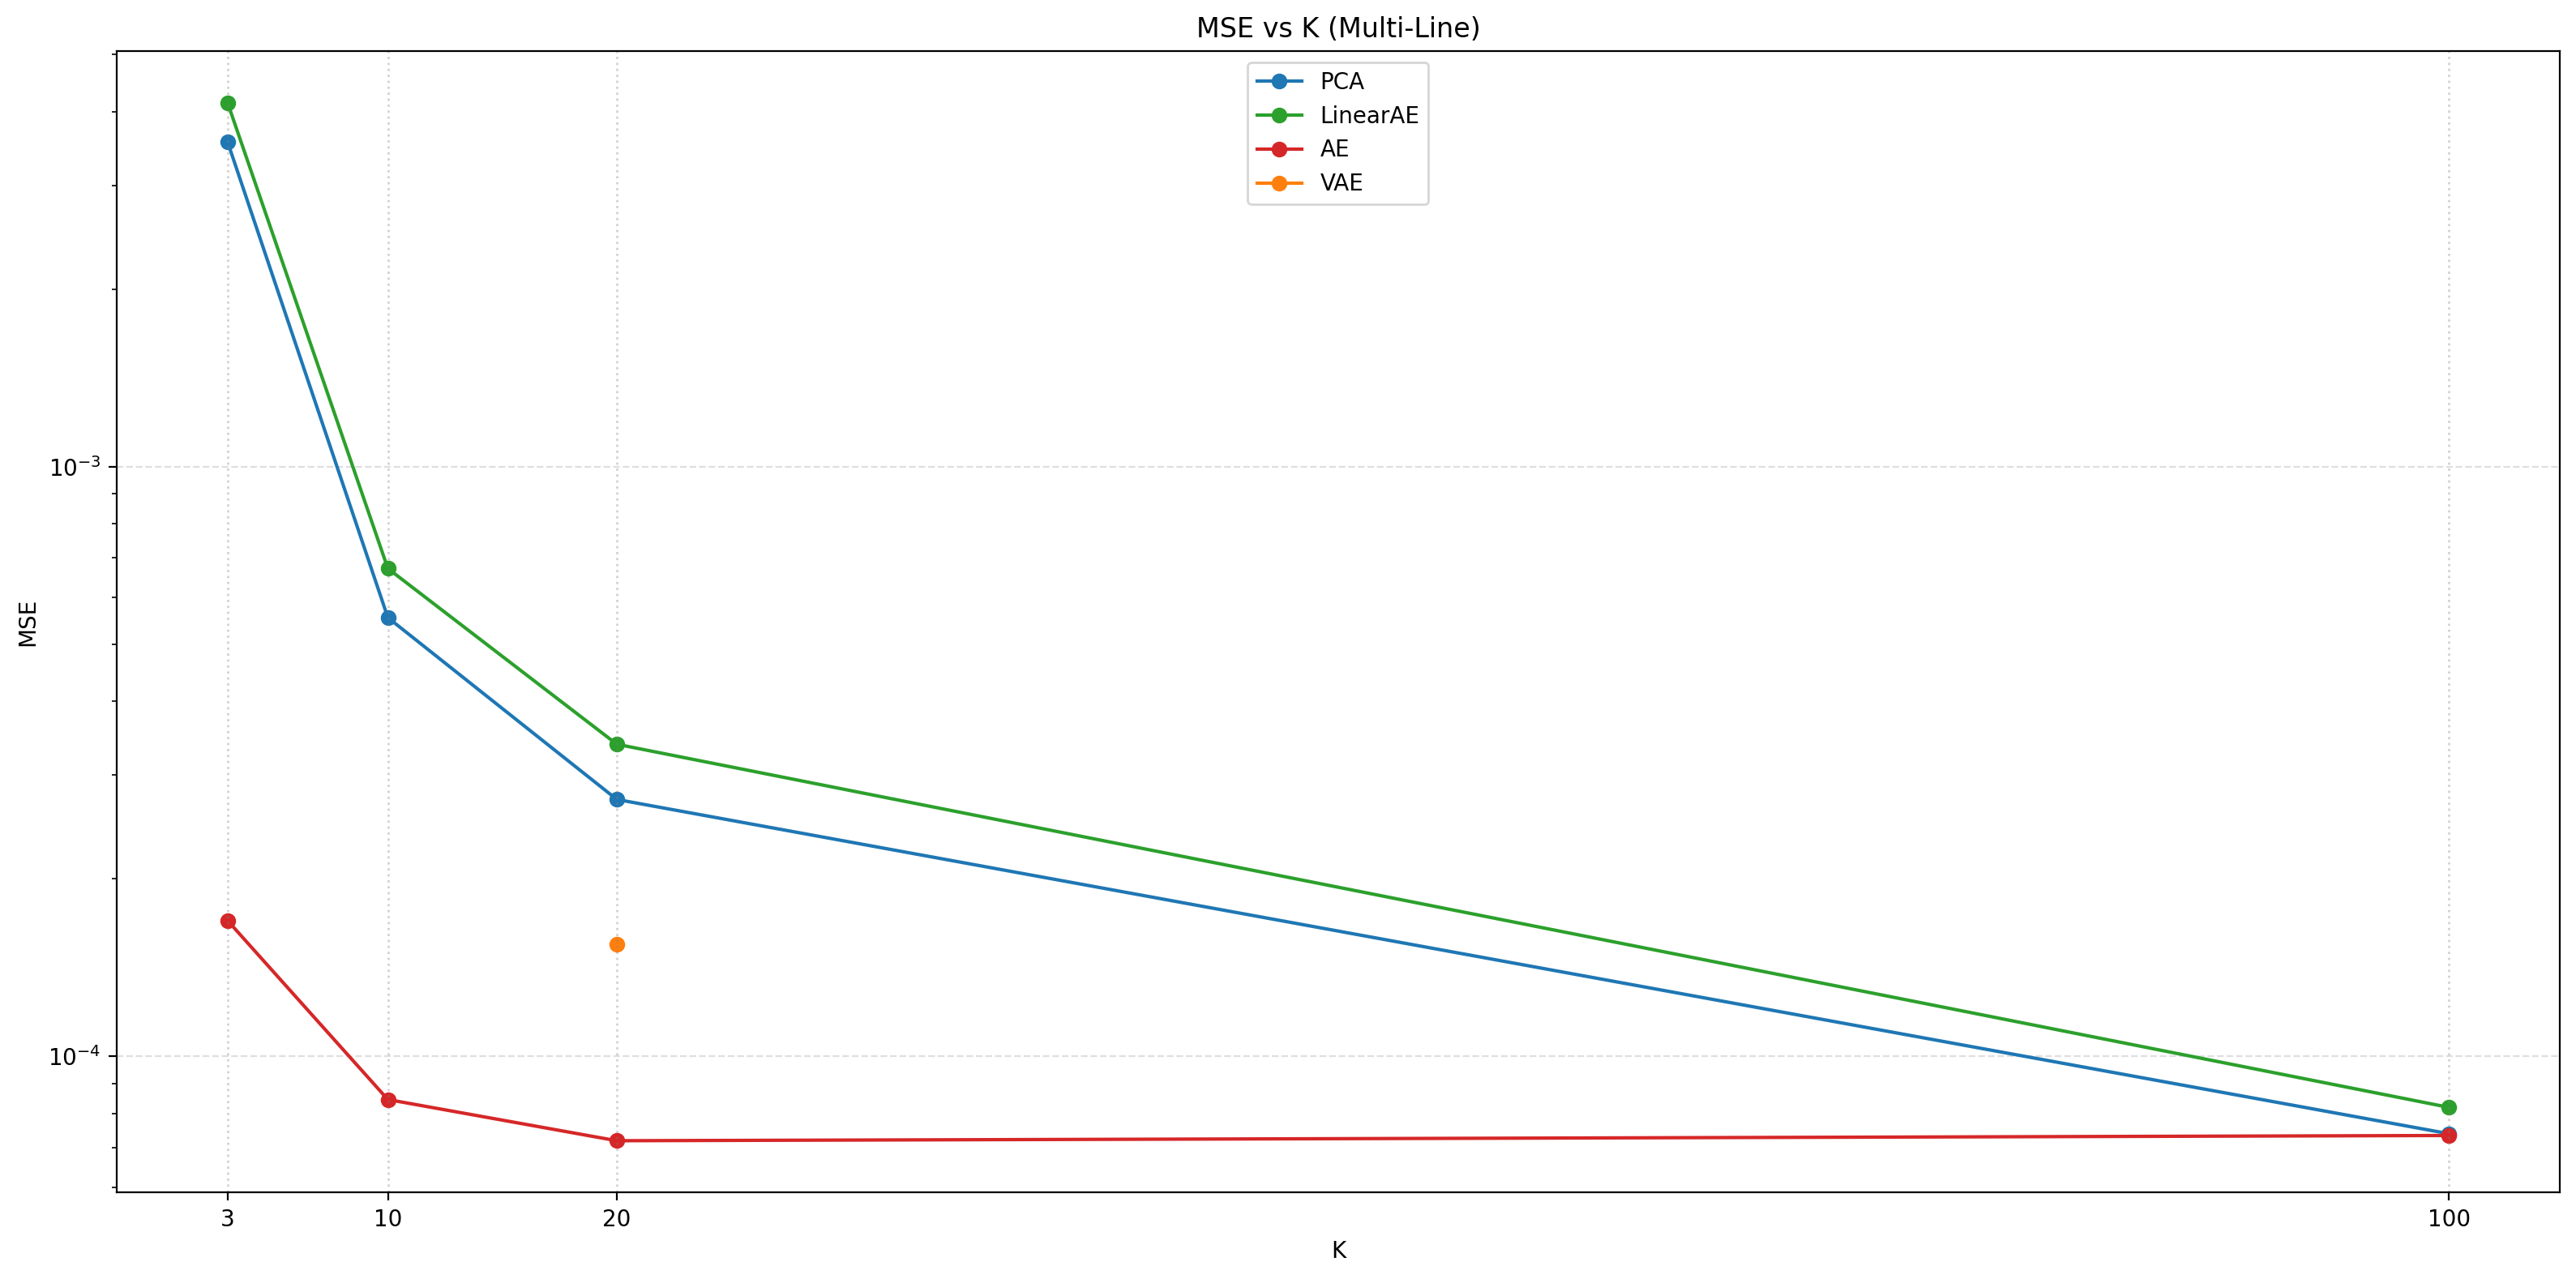
\includegraphics[width=0.75\textwidth]{./Pictures/capitolo7/fig_mse_vs_k.png}
\caption{MSE di ricostruzione sul \emph{Test Set} (dominio Cholesky) in funzione della dimensione latente $K$, per i quattro modelli confrontati (scala logaritmica).}
\label{fig:mse_vs_k}
\end{figure}

Tuttavia, l'analisi dell'errore di ricostruzione sul \emph{Test Set} (Figura~\ref{fig:mse_vs_k}) rivela il limite strutturale di questi approcci: a ogni valore di $K$, sia la PCA sia il Linear AE restano nettamente al di sopra dell'errore dell'Autoencoder Profondo (Sezione~\ref{sec:risultati_ae_vae}). La rigidità dell'iperpiano di proiezione impedisce ai modelli lineari di adattarsi alle complesse interdipendenze non lineari che governano le rotazioni settoriali e le asimmetrie strutturali tra diversi regimi di mercato. La PCA comprime l'informazione in modo algebricamente efficiente, ma restituisce una ricostruzione storicamente "appiattita", faticando a preservare la complessa microstruttura dei veri \emph{stylized facts} finanziari.

\section{Performance di ricostruzione: AE Non-Lineare e VAE}
\label{sec:risultati_ae_vae}

L'introduzione della non-linearità attraverso l'Autoencoder Profondo (Deep AE) ha prodotto un netto superamento del limite imposto dalla PCA, sia sul \emph{Training Set} sia, cosa più rilevante, sul \emph{Test Set} mai visto durante l'addestramento (Tabella~\ref{tab:mse_test_cholesky} e Figura~\ref{fig:mse_vs_k}): a $K=20$, ad esempio, l'MSE di test dell'AE ($7.19\times10^{-5}$) è di quasi quattro volte inferiore a quello della PCA ($2.73\times10^{-4}$). Questo risultato è reso possibile dall'omogeneizzazione statistica introdotta dal campionamento a mescolamento casuale (Capitolo~\ref{ch:preprocessing}): a differenza di quanto osservato nei test preliminari con partizionamento temporale sequenziale (dove il \emph{distribution shift} tra regimi macroeconomici impediva ai modelli non lineari di generalizzare, portandoli persino a essere superati dalla PCA), nella pipeline definitiva l'Autoencoder Profondo non mostra segni di \emph{overfitting}: \emph{Training Loss} e \emph{Validation/Test Loss} rimangono stabilmente allineate su tutto l'arco di $K$ testati.

Il passaggio al Variational Autoencoder (VAE) introduce una dinamica prestazionale più sfumata di quanto una prima intuizione potrebbe suggerire. Il VAE, addestrato nella parametrizzazione Cholesky con la \emph{Reconstruction Loss} basata sulla Divergenza di Jeffreys (Sezione~\ref{sec:setup_vae}), ottiene a $K=20$ un MSE di test pari a $1.55\times10^{-4}$, \textbf{inferiore} sia a quello della PCA ($2.73\times10^{-4}$) sia a quello del Linear AE ($3.38\times10^{-4}$), pur restando superiore a quello dell'Autoencoder Profondo deterministico ($7.19\times10^{-5}$).

\begin{table}[h!]
\centering
\begin{tabular}{lrrrr}
\hline
\textbf{Metrica MST ($K=20$, Test)} & PCA & Linear AE & AE & VAE \\
\hline
\emph{Edge overlap} (\%) & 83.0 & 83.1 & 91.1 & 88.4 \\
\emph{Edge Jaccard} (\%) & 71.2 & 71.4 & 84.0 & 79.4 \\
Distanza $L_1$ distribuzione di grado & 0.081 & 0.084 & 0.068 & 0.076 \\
\emph{Betweenness} \emph{top-10} overlap (\%) & 71.7 & 68.6 & 80.2 & 77.9 \\
\hline
\end{tabular}
\caption{Metriche topologiche di similarità del Minimum Spanning Tree tra matrice originale e ricostruita, dominio Cholesky, $K=20$, \emph{Test Set}. Il VAE non è mai stato confrontato a $K=3$ o $K=100$: si vedano le Osservazioni a fine sezione.}
\label{tab:mst_test_cholesky}
\end{table}

\begin{figure}[h!]
\centering
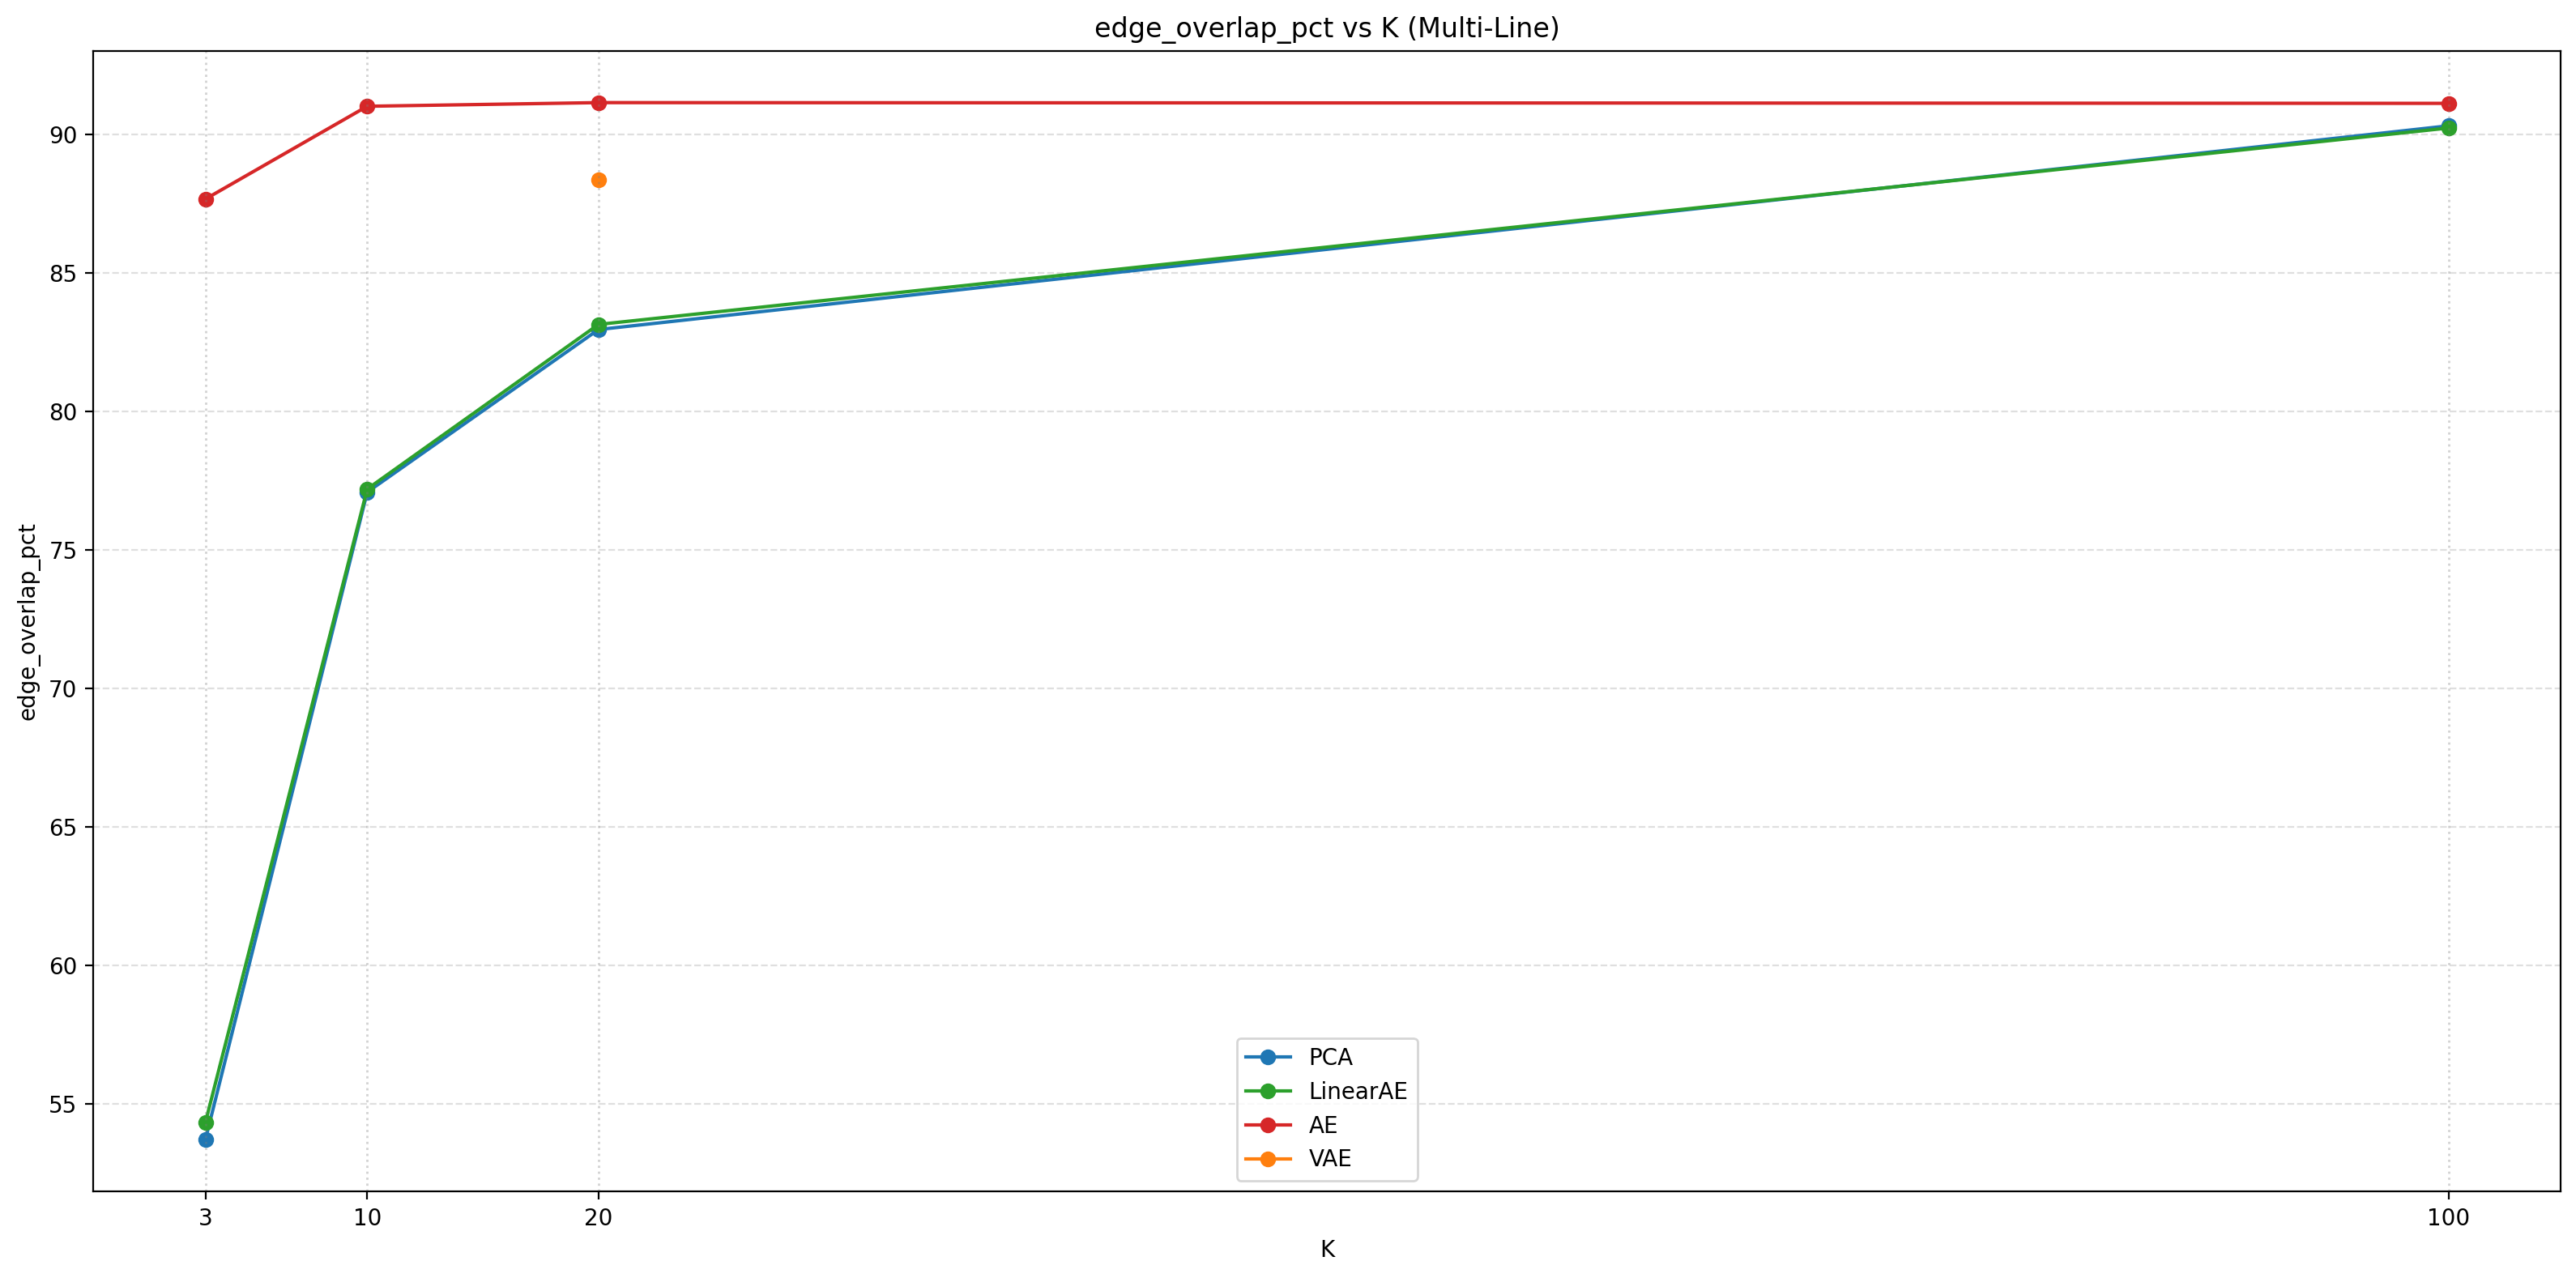
\includegraphics[width=0.75\textwidth]{./Pictures/capitolo7/fig_mst_edge_overlap_vs_k.png}
\caption{Percentuale di archi in comune tra l'MST della matrice originale e quello della matrice ricostruita, dominio Cholesky, \emph{Test Set}, in funzione di $K$.}
\label{fig:mst_edge_overlap_vs_k}
\end{figure}

Le metriche topologiche basate sul Minimum Spanning Tree (Tabella~\ref{tab:mst_test_cholesky} e Figura~\ref{fig:mst_edge_overlap_vs_k}) confermano lo stesso ordinamento: l'Autoencoder Profondo preserva la topologia di rete meglio di tutti gli altri modelli a ogni $K$; il VAE si colloca sistematicamente in posizione intermedia, superando nettamente PCA e Linear AE pur non raggiungendo la fedeltà topologica dell'AE deterministico.

Questo risultato non è casuale, ma la diretta conseguenza della natura della \emph{Reconstruction Loss} impiegata: la loss basata sulla Divergenza di Jeffreys (Sezione~\ref{sec:setup_vae}) pesa esplicitamente l'errore sulla struttura spettrale della matrice di correlazione ricostruita, anziché limitarsi a un errore elemento-per-elemento sui coefficienti del fattore di Cholesky; questa parametrizzazione più informativa, unita alla garanzia strutturale di PSD, riduce significativamente il costo che il vincolo di regolarizzazione $D_{KL}$ impone alla fedeltà di ricostruzione.

\begin{osservazione}
Il confronto a $K=20$ presentato in questa sezione è l'unico punto in cui tutti e quattro i modelli sono stati valutati sullo stesso \emph{Test Set} con la stessa metodologia. Il VAE non è stato sistematicamente confrontato a $K=3$ o $K=100$; inoltre l'errore di ricostruzione del VAE, a differenza degli altri tre modelli, non decresce monotonicamente con $K$ (MSE sul \emph{Training Set}: $6.33\times10^{-5}$ a $K=10$, $8.69\times10^{-5}$ a $K=20$, $1.16\times10^{-4}$ a $K=30$) --- un andamento anomalo, verosimilmente legato alla competizione tra ricostruzione e regolarizzazione KL e al fatto che le run confrontate a $K=10,20,30$ non condividono esattamente gli stessi iperparametri di addestramento (non è quindi un \emph{ablation study} controllato sul solo $K$).
\end{osservazione}

\section{Il trade-off tra compressione esatta e flessibilità generativa}
\label{sec:tradeoff_generazione}

I risultati finora descritti delineano il compromesso fondamentale che giustifica l'adozione delle architetture variazionali in finanza quantitativa. Non si tratta, come i risultati del dominio Cholesky dimostrano, di una dicotomia netta tra "il VAE ricostruisce peggio di tutto" e "il VAE genera scenari realistici": il VAE resta competitivo, e anzi superiore, ai \emph{benchmark} lineari anche in pura ricostruzione. Il compromesso reale è più circoscritto, e riguarda specificamente il confronto tra Autoencoder Profondo deterministico e VAE.

L'Autoencoder Profondo deterministico massimizza l'efficacia della compressione storica (Sezione~\ref{sec:risultati_ae_vae}), ma fallisce totalmente qualora lo si voglia utilizzare come motore di simulazione. Poiché lo spazio latente di un AE classico non è governato da alcuna restrizione probabilistica, i vettori $\mathbf{z}$ si dispongono in modo disaggregato e frammentario, creando vaste regioni di vuoto geometrico (Capitolo~\ref{ch:modelli_generativi}, \S\ref{sec:deep_ae}). Tentare di generare nuovi scenari campionando un vettore casuale da tale spazio e proiettandolo attraverso il \emph{Decoder} produce output privi di coerenza economico-finanziaria. L'AE deterministico è quindi confinato alla pura memorizzazione di un passato statico, per quanto accurata.

Il VAE, pur restando lievemente meno accurato dell'AE nella pura ricostruzione (Tabella~\ref{tab:mse_test_cholesky}), paga questo scarto --- contenuto, e non catastrofico come inizialmente ipotizzato --- in cambio dell'unica proprietà che rende possibile la generazione stocastica: un vincolo di regolarizzazione ($D_{KL}$) che modella uno spazio latente continuo, denso e privo di singolarità, in cui è possibile campionare in modo significativo (Capitolo~\ref{ch:modelli_generativi}, \S\ref{sec:vae}). È proprio questa capacità generativa, resa possibile senza rinunciare in modo sostanziale alla fedeltà di ricostruzione, a motivare la scelta del VAE come modello finale per la generazione di scenari sintetici affrontata nel Capitolo~\ref{ch:generazione_stocastica}, dove la procedura di campionamento effettivamente adottata (un \emph{block-bootstrap} storico nello spazio latente) e la validazione delle matrici generate sui cinque fatti stilizzati del Capitolo~\ref{ch:stylized_facts} vengono presentate in dettaglio.

% \chapter{Generazione Stocastica di Nuovi Scenari (Validazione del VAE)}
\label{ch:generazione_stocastica}

\section{Campionamento dallo spazio latente: dal prior al block-bootstrap storico}
\label{sec:block_bootstrap}

Come discusso nel Capitolo~\ref{ch:modelli_generativi} (\S\ref{sec:vae}), la regolarizzazione imposta dalla Divergenza di Kullback-Leibler rende in linea di principio possibile generare nuove matrici di correlazione campionando direttamente un vettore casuale $\mathbf{z}_{\text{sim}} \sim \mathcal{N}(\mathbf{0}, \mathbf{I})$ dal \emph{prior} e decodificandolo. Tuttavia, l'obiettivo di questo lavoro non è produrre uno scenario plausibile qualsiasi, bensì \textbf{prevedere la struttura di correlazione a un orizzonte di un mese} a partire dallo stato di mercato osservato oggi (Capitolo~\ref{ch:matrici_finanziarie}, \S\ref{sec:markowitz}). Per questo motivo, la procedura di generazione effettivamente adottata sostituisce il semplice campionamento dal \emph{prior} con una tecnica di \textbf{block-bootstrap storico nello spazio latente}, che ancora la generazione stocastica alla dinamica recente del mercato pur sfruttando la medesima regolarità topologica dello spazio latente descritta nel Capitolo~\ref{ch:modelli_generativi}.

La procedura, applicata al modello VAE a 20 dimensioni latenti nel dominio Cholesky con loss di Jeffreys (\texttt{VAE\_20dim\_cholesky\_06\_loss}, lo stesso modello impiegato per il confronto del Capitolo~\ref{ch:analisi_compressione}), si articola nei seguenti passaggi:
\begin{enumerate}
    \item \textbf{Ricostruzione della traiettoria latente storica.} L'encoder del VAE già addestrato viene applicato all'intera serie storica delle matrici di correlazione calcolate con passo giornaliero ($\text{stride}=1$, a differenza dello stride di 10 giorni usato per l'addestramento, si veda il Capitolo~\ref{ch:preprocessing}), producendo una traiettoria latente continua $\{\mathbf{z}_t\}_{t=1}^{T}$ con $T=4124$ osservazioni giornaliere.
    \item \textbf{Calcolo degli incrementi giornalieri.} Si calcola la sequenza degli incrementi $\Delta\mathbf{z}_t = \mathbf{z}_t - \mathbf{z}_{t-1}$, che rappresenta la variazione giorno-su-giorno osservata nello spazio latente durante l'intero periodo storico.
    \item \textbf{Campionamento a blocchi.} Per generare ciascuno scenario sintetico, si estrae casualmente un blocco di 21 incrementi giornalieri consecutivi (corrispondenti a un mese lavorativo) dalla sequenza storica $\{\Delta\mathbf{z}_t\}$ e se ne calcola la somma cumulata $\delta\mathbf{z}$.
    \item \textbf{Proiezione a un mese.} Il salto latente campionato viene sommato allo stato attuale $\mathbf{z}_{\text{oggi}}$ (l'ultima osservazione della traiettoria storica), ottenendo lo stato latente previsto $\mathbf{z}_{\text{futuro}} = \mathbf{z}_{\text{oggi}} + \delta\mathbf{z}$.
    \item \textbf{Decodifica e ricostruzione PSD.} Il Decoder produce il fattore di Cholesky corrispondente a $\mathbf{z}_{\text{futuro}}$, da cui si ricostruisce la matrice di correlazione sintetica tramite $\mathbf{C} = \mathbf{L}\mathbf{L}^T$ e normalizzazione, garantendone la semidefinita positività per costruzione (Capitolo~\ref{ch:modelli_generativi}, \S\ref{sec:vae}).
\end{enumerate}

Ripetendo il campionamento a blocchi un numero $N$ di volte (in questo lavoro, $N=100$ e $N=1000$), si ottiene un insieme di scenari sintetici a un mese di distanza, ciascuno ancorato allo stesso stato di partenza $\mathbf{z}_{\text{oggi}}$ ma diversificato dalla variabilità storica campionata a blocchi.

\begin{figure}[h!]
\centering
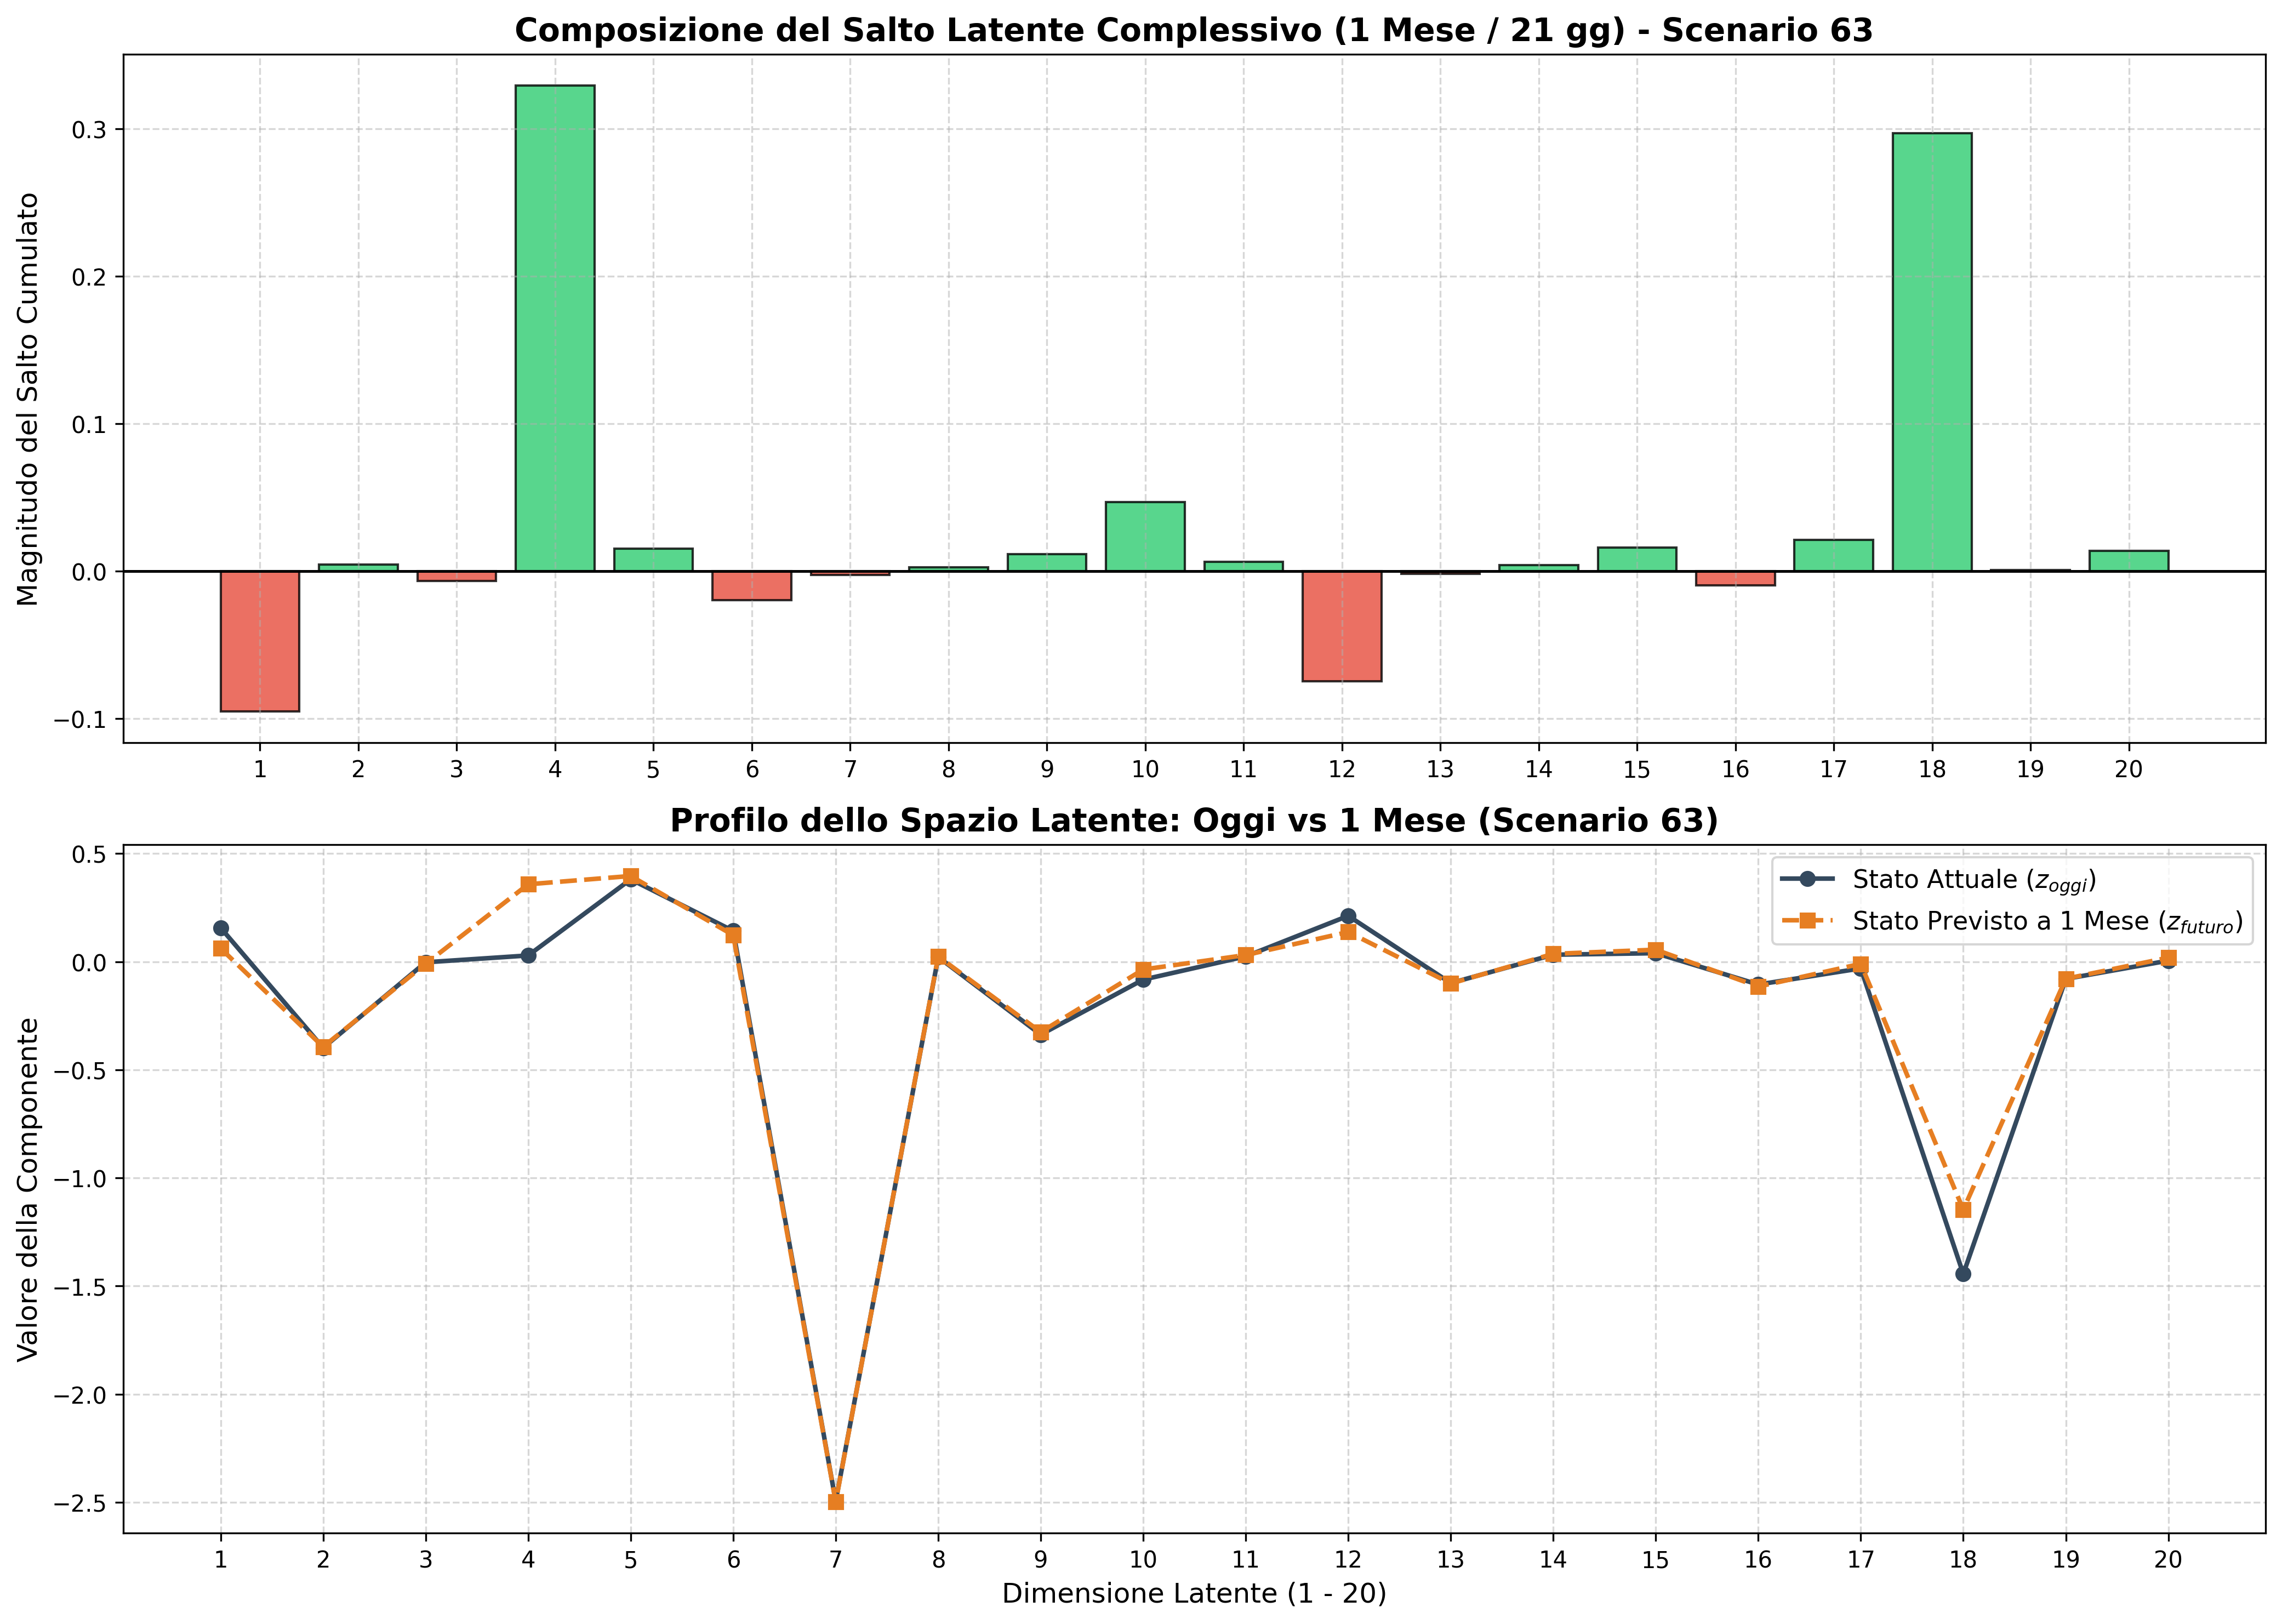
\includegraphics[width=0.85\textwidth]{./Pictures/capitolo8/fig_block_bootstrap_latente.png}
\caption{Illustrazione della procedura di block-bootstrap per uno scenario sintetico (\emph{Scenario 63} tra i 1000 generati): in alto, la composizione del salto latente cumulato sulle 20 dimensioni; in basso, il confronto tra lo stato attuale $\mathbf{z}_{\text{oggi}}$ e lo stato previsto a un mese $\mathbf{z}_{\text{futuro}}$.}
\label{fig:block_bootstrap}
\end{figure}

La Figura~\ref{fig:block_bootstrap} illustra la composizione del salto latente per uno degli scenari generati: si osserva come solo alcune dimensioni latenti (tipicamente 2--4 su 20) contribuiscano in modo sostanziale allo spostamento complessivo, mentre le restanti rimangono pressoché invariate rispetto allo stato attuale --- un comportamento coerente con la struttura dello spazio latente appreso dal VAE, in cui poche direzioni concentrano la maggior parte della variabilità informativa del mercato.

\section{Verifica dei cinque fatti stilizzati sulle matrici generate}
\label{sec:verifica_stylized_facts_generate}

Per validare la plausibilità economico-finanziaria delle matrici sintetiche prodotte, ciascuno scenario generato viene confrontato con la matrice di correlazione osservata oggi sulla base dei cinque fatti stilizzati introdotti nel Capitolo~\ref{ch:stylized_facts}. Lo scenario qui presentato in dettaglio (\emph{Scenario 63}, tra i 1000 generati dal modello \texttt{VAE\_20dim\_cholesky\_06\_loss}) è stato scelto perché si colloca al 95\textdegree\ percentile lungo il primo asse principale della nuvola di scenari generati (che spiega il 23.4\% della varianza totale, Figura~\ref{fig:analisi_statistica}): non è quindi uno scenario arbitrario o "comodo", ma uno scenario di coda, rappresentativo di una plausibile evoluzione di mercato relativamente pronunciata rispetto allo stato attuale.

\begin{figure}[h!]
\centering
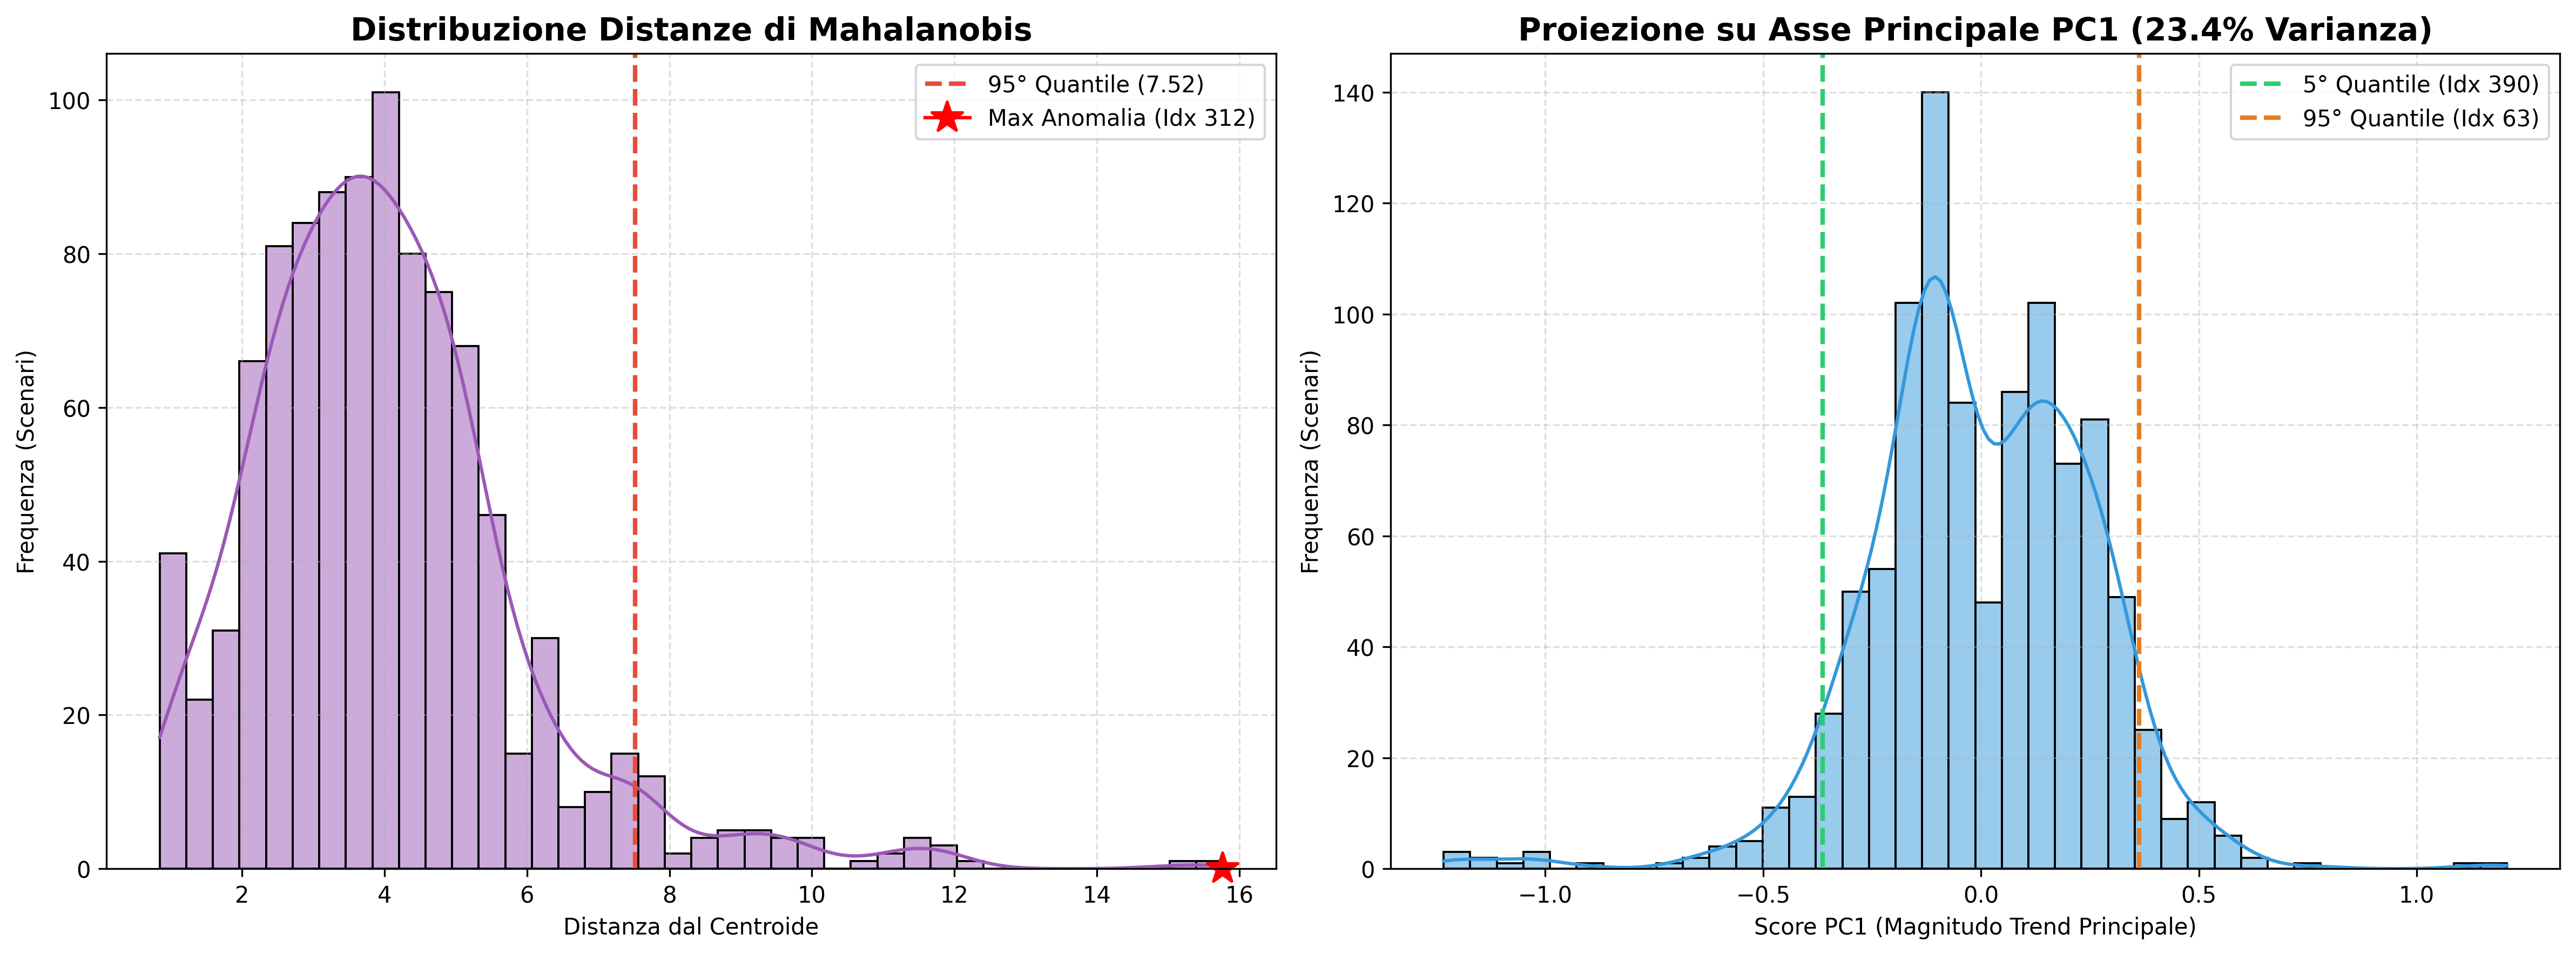
\includegraphics[width=0.95\textwidth]{./Pictures/capitolo8/fig_analisi_statistica_1000_scenari.png}
\caption{Analisi statistica della nuvola di 1000 scenari generati: distribuzione delle distanze di Mahalanobis dal centroide (sinistra) e proiezione sul primo asse principale (destra). Lo Scenario 63, oggetto dell'analisi di dettaglio, si colloca al 95\textdegree\ percentile lungo il primo asse.}
\label{fig:analisi_statistica}
\end{figure}

\paragraph{Distribuzione pairwise.} La distribuzione dei coefficienti di correlazione dello scenario sintetico (Figura~\ref{fig:pairwise_generato}) mantiene lo spostamento verso valori positivi osservato nel mercato reale: media $0.4635$ e mediana $0.4711$ per lo scenario generato, contro $0.4512$ e $0.4593$ della matrice odierna --- coerenti, per ordine di grandezza, con quanto verificato sulla matrice di esempio analizzata nel Capitolo~\ref{ch:stylized_facts}.

\begin{figure}[h!]
\centering
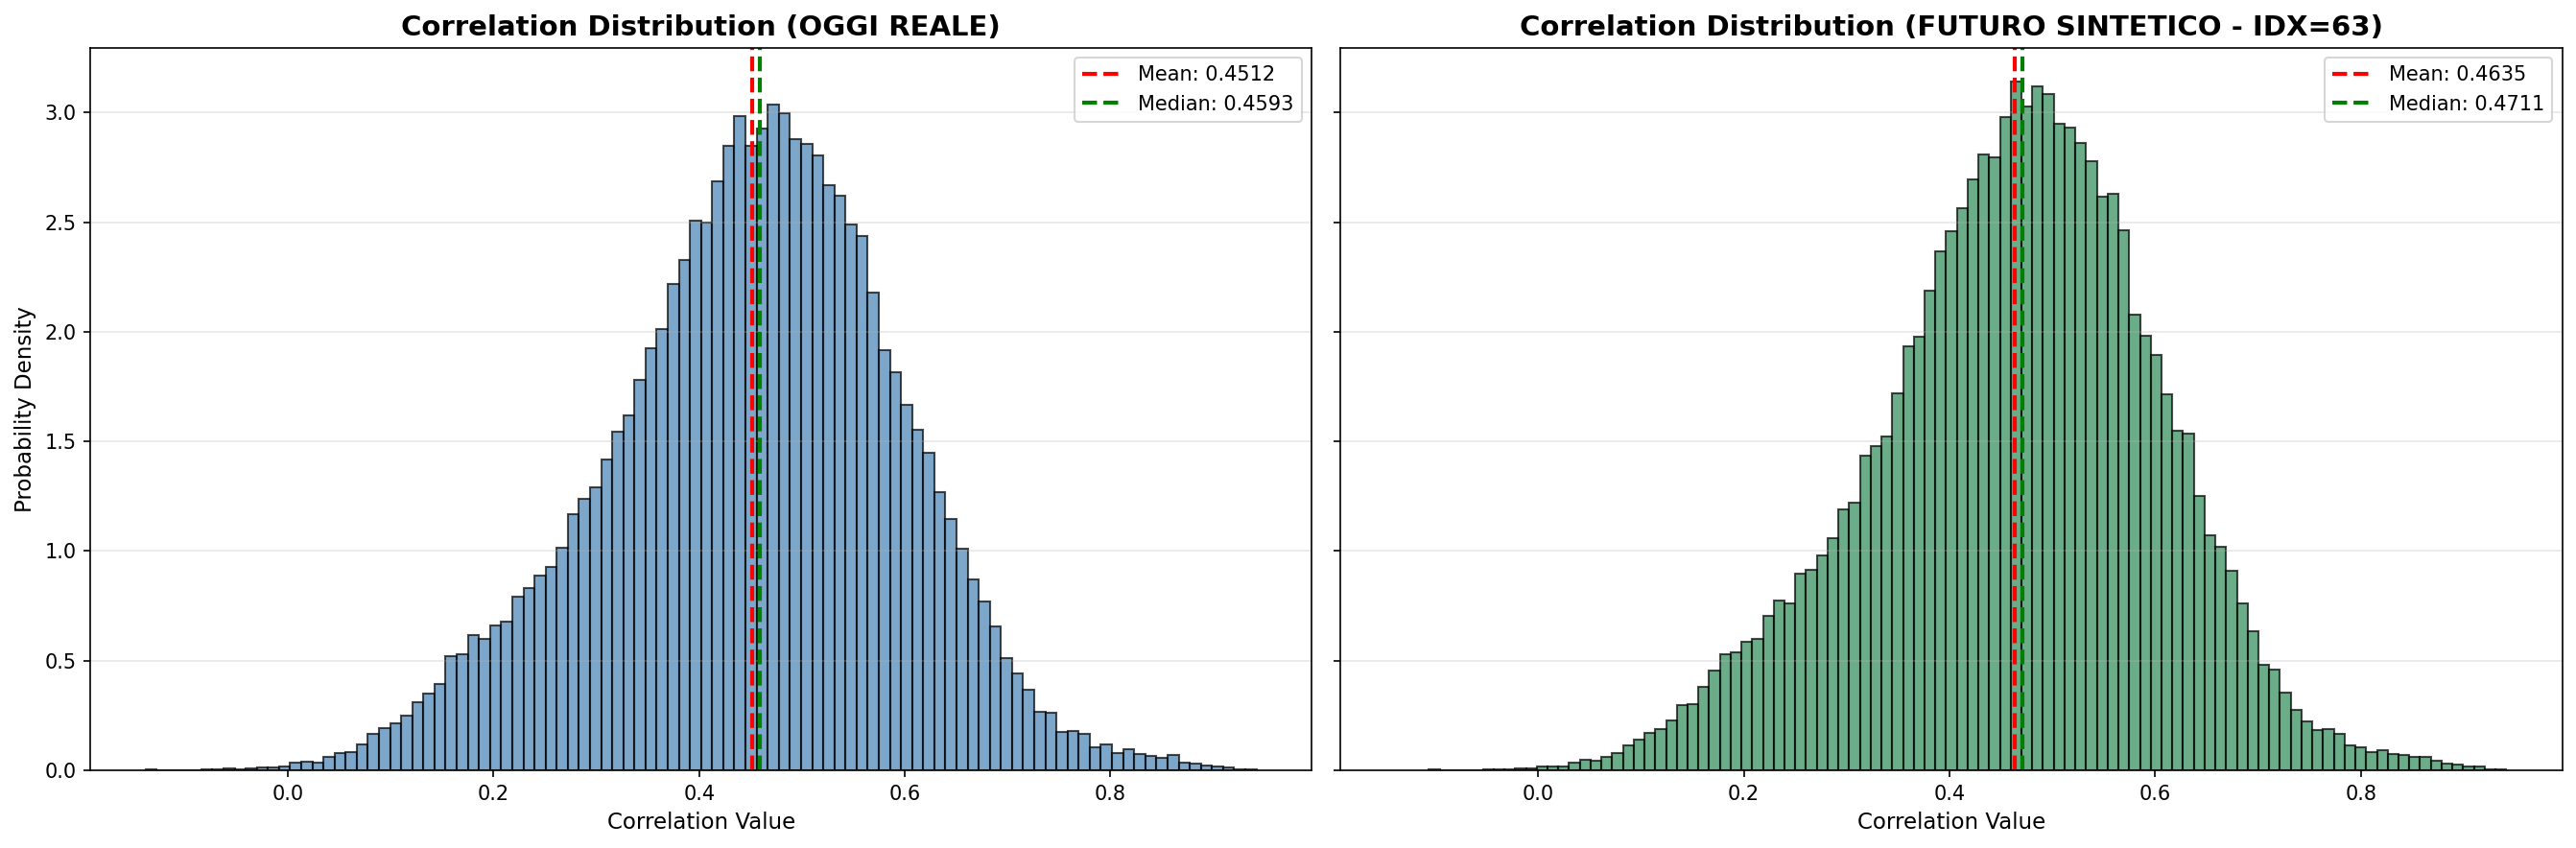
\includegraphics[width=0.95\textwidth]{./Pictures/capitolo8/fig_pairwise_distribution_generato.png}
\caption{Confronto tra la distribuzione dei coefficienti \emph{pairwise} della matrice odierna (sinistra) e della matrice sintetica a un mese (destra).}
\label{fig:pairwise_generato}
\end{figure}

\paragraph{Spettro e distribuzione di Marchenko-Pastur.} Lo spettro della matrice generata (Figura~\ref{fig:mp_generato}) preserva la struttura a tre componenti descritta nel Capitolo~\ref{ch:stylized_facts}: l'autovalore di mercato rimane dominante e di ordine di grandezza confrontabile ($169.1$ per la matrice odierna, $173.2$ per lo scenario generato), e lo stesso numero di autovalori settoriali (nove) supera il limite superiore teorico di Marchenko-Pastur in entrambe le matrici.

\begin{figure}[h!]
\centering
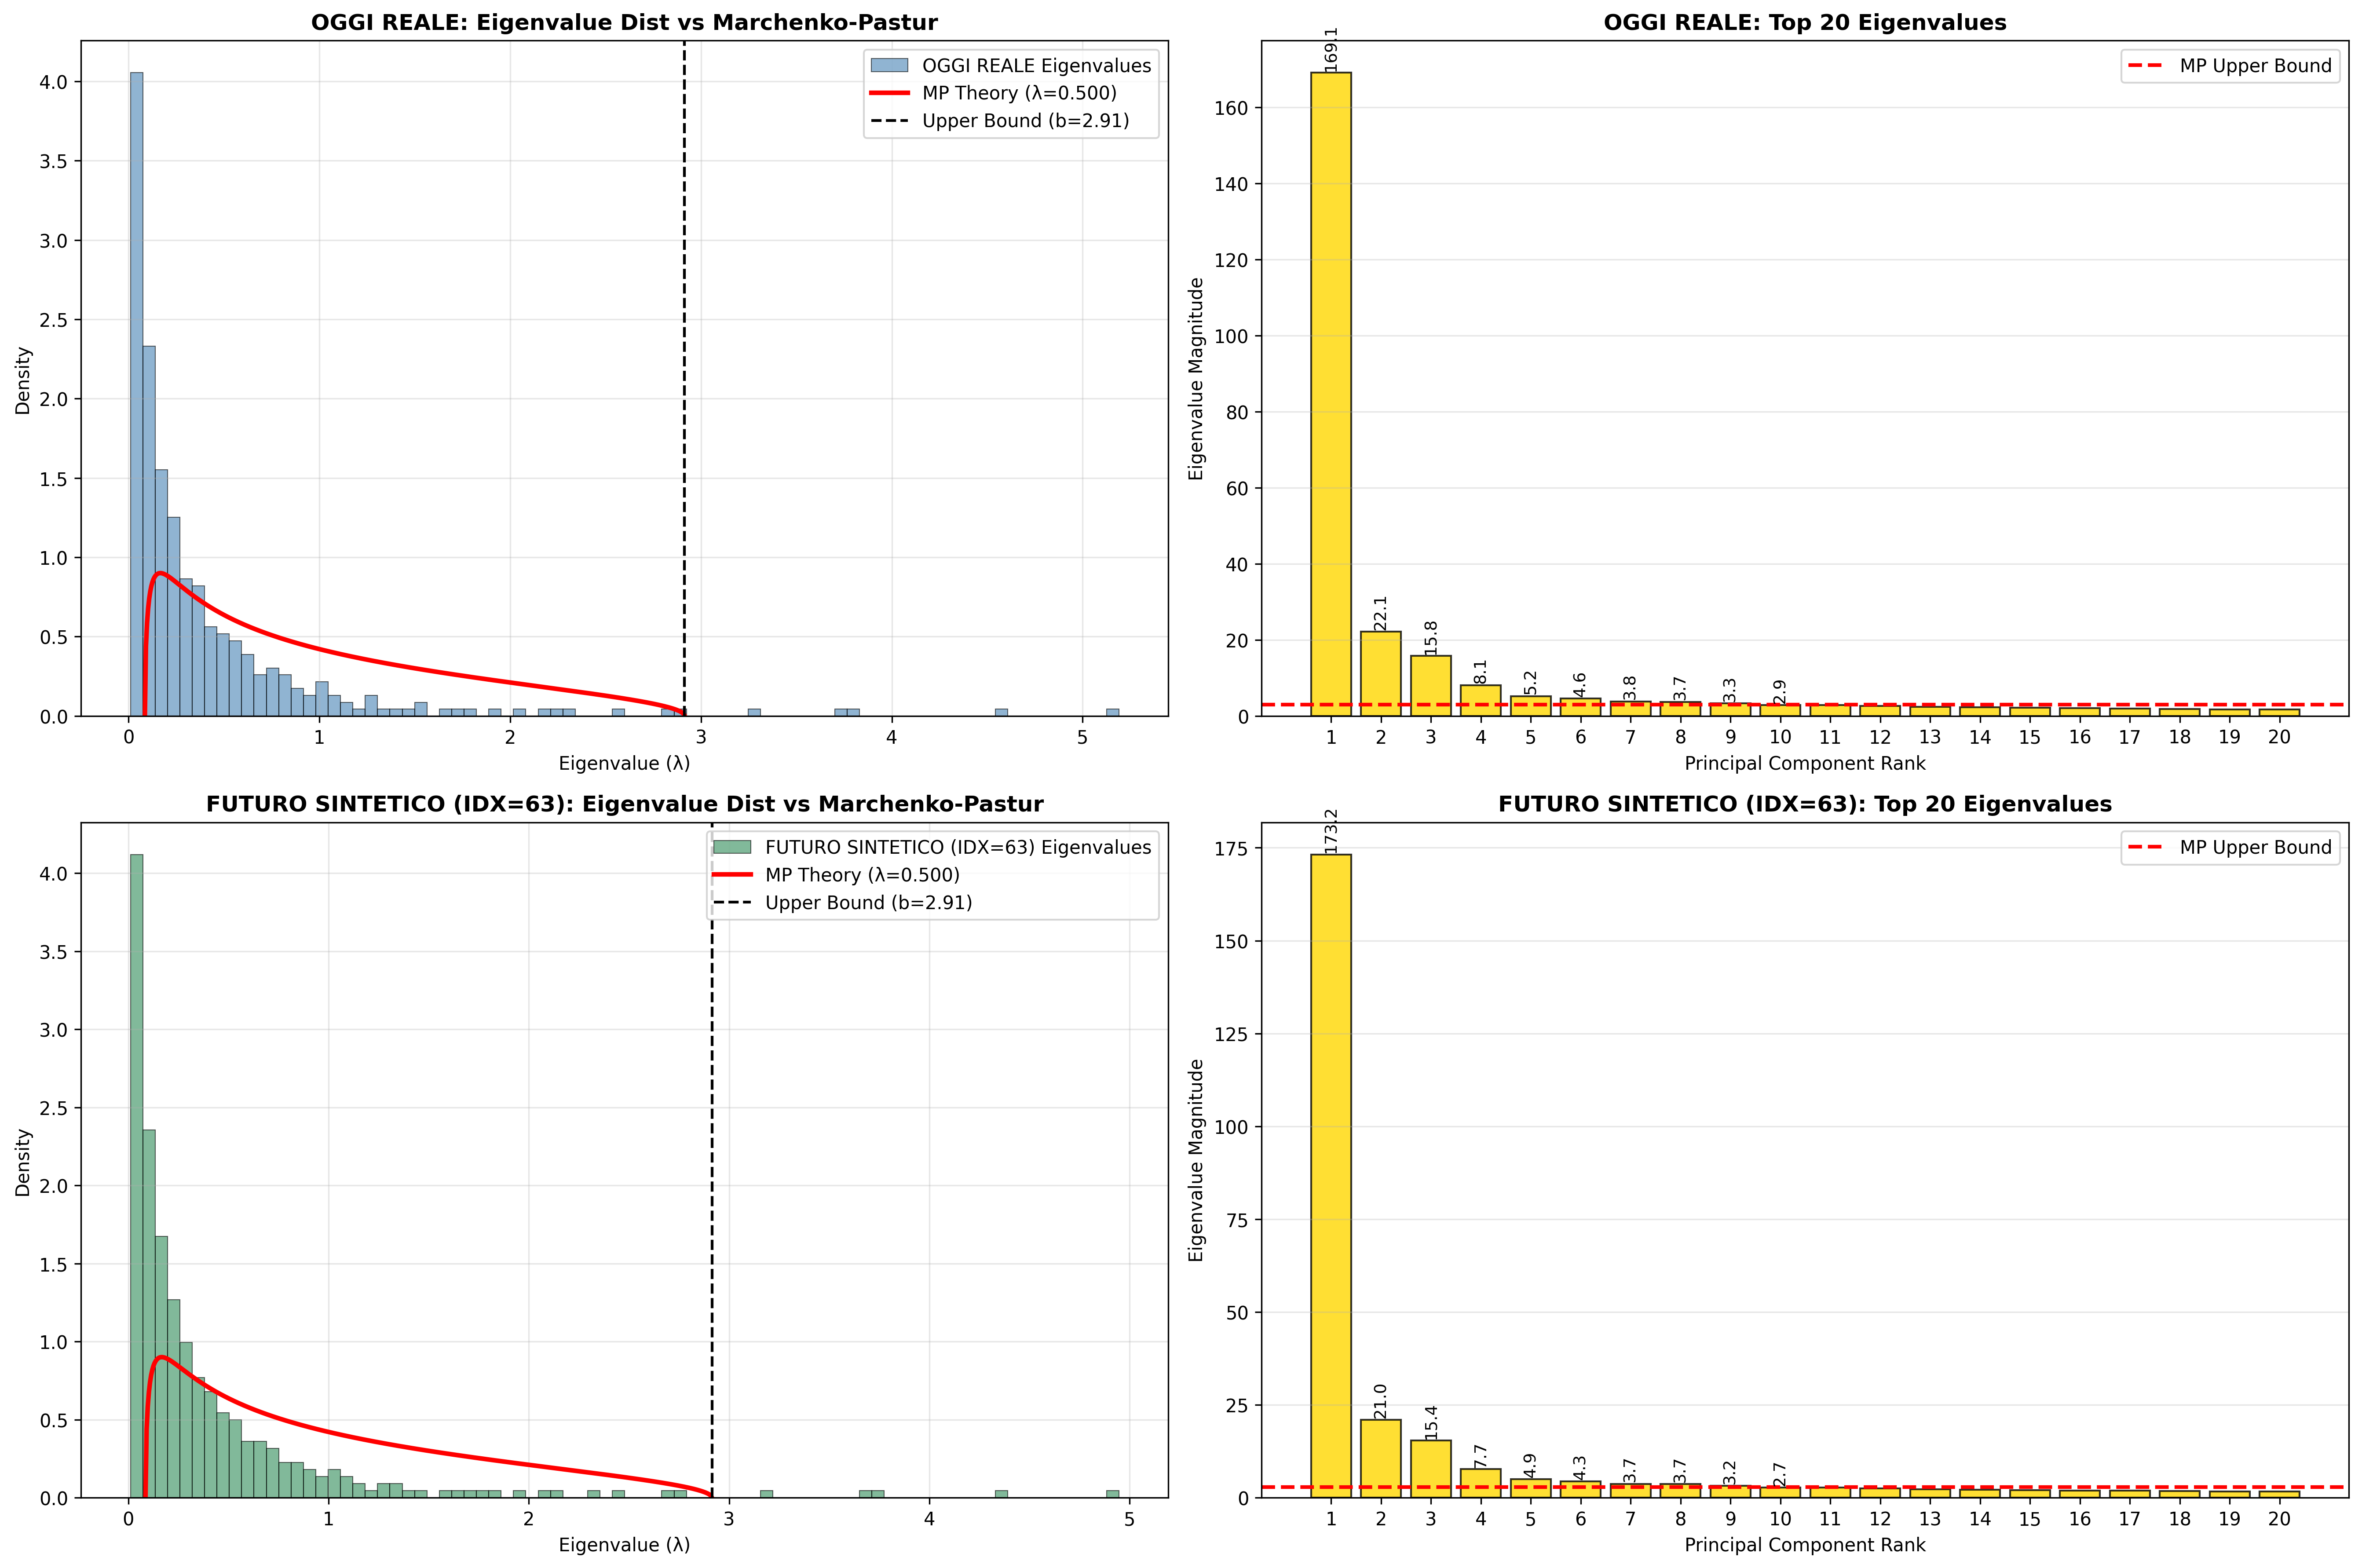
\includegraphics[width=0.95\textwidth]{./Pictures/capitolo8/fig_marchenko_pastur_generato.png}
\caption{Spettro degli autovalori della matrice odierna (in alto) e della matrice sintetica (in basso) confrontato con la distribuzione teorica di Marchenko-Pastur.}
\label{fig:mp_generato}
\end{figure}

\paragraph{Proprietà di Perron-Frobenius.} Il primo autovettore (\emph{market mode}) della matrice sintetica presenta componenti tutte dello stesso segno, in accordo con la proprietà di Perron-Frobenius, con una similarità coseno rispetto all'autovettore della matrice odierna pari a $0.9999$ (Figura~\ref{fig:pf_generato}); anche il secondo e il terzo autovettore (\emph{sector mode}) risultano preservati con similarità coseno rispettivamente di $0.9893$ e $0.9883$.

\begin{figure}[h!]
\centering
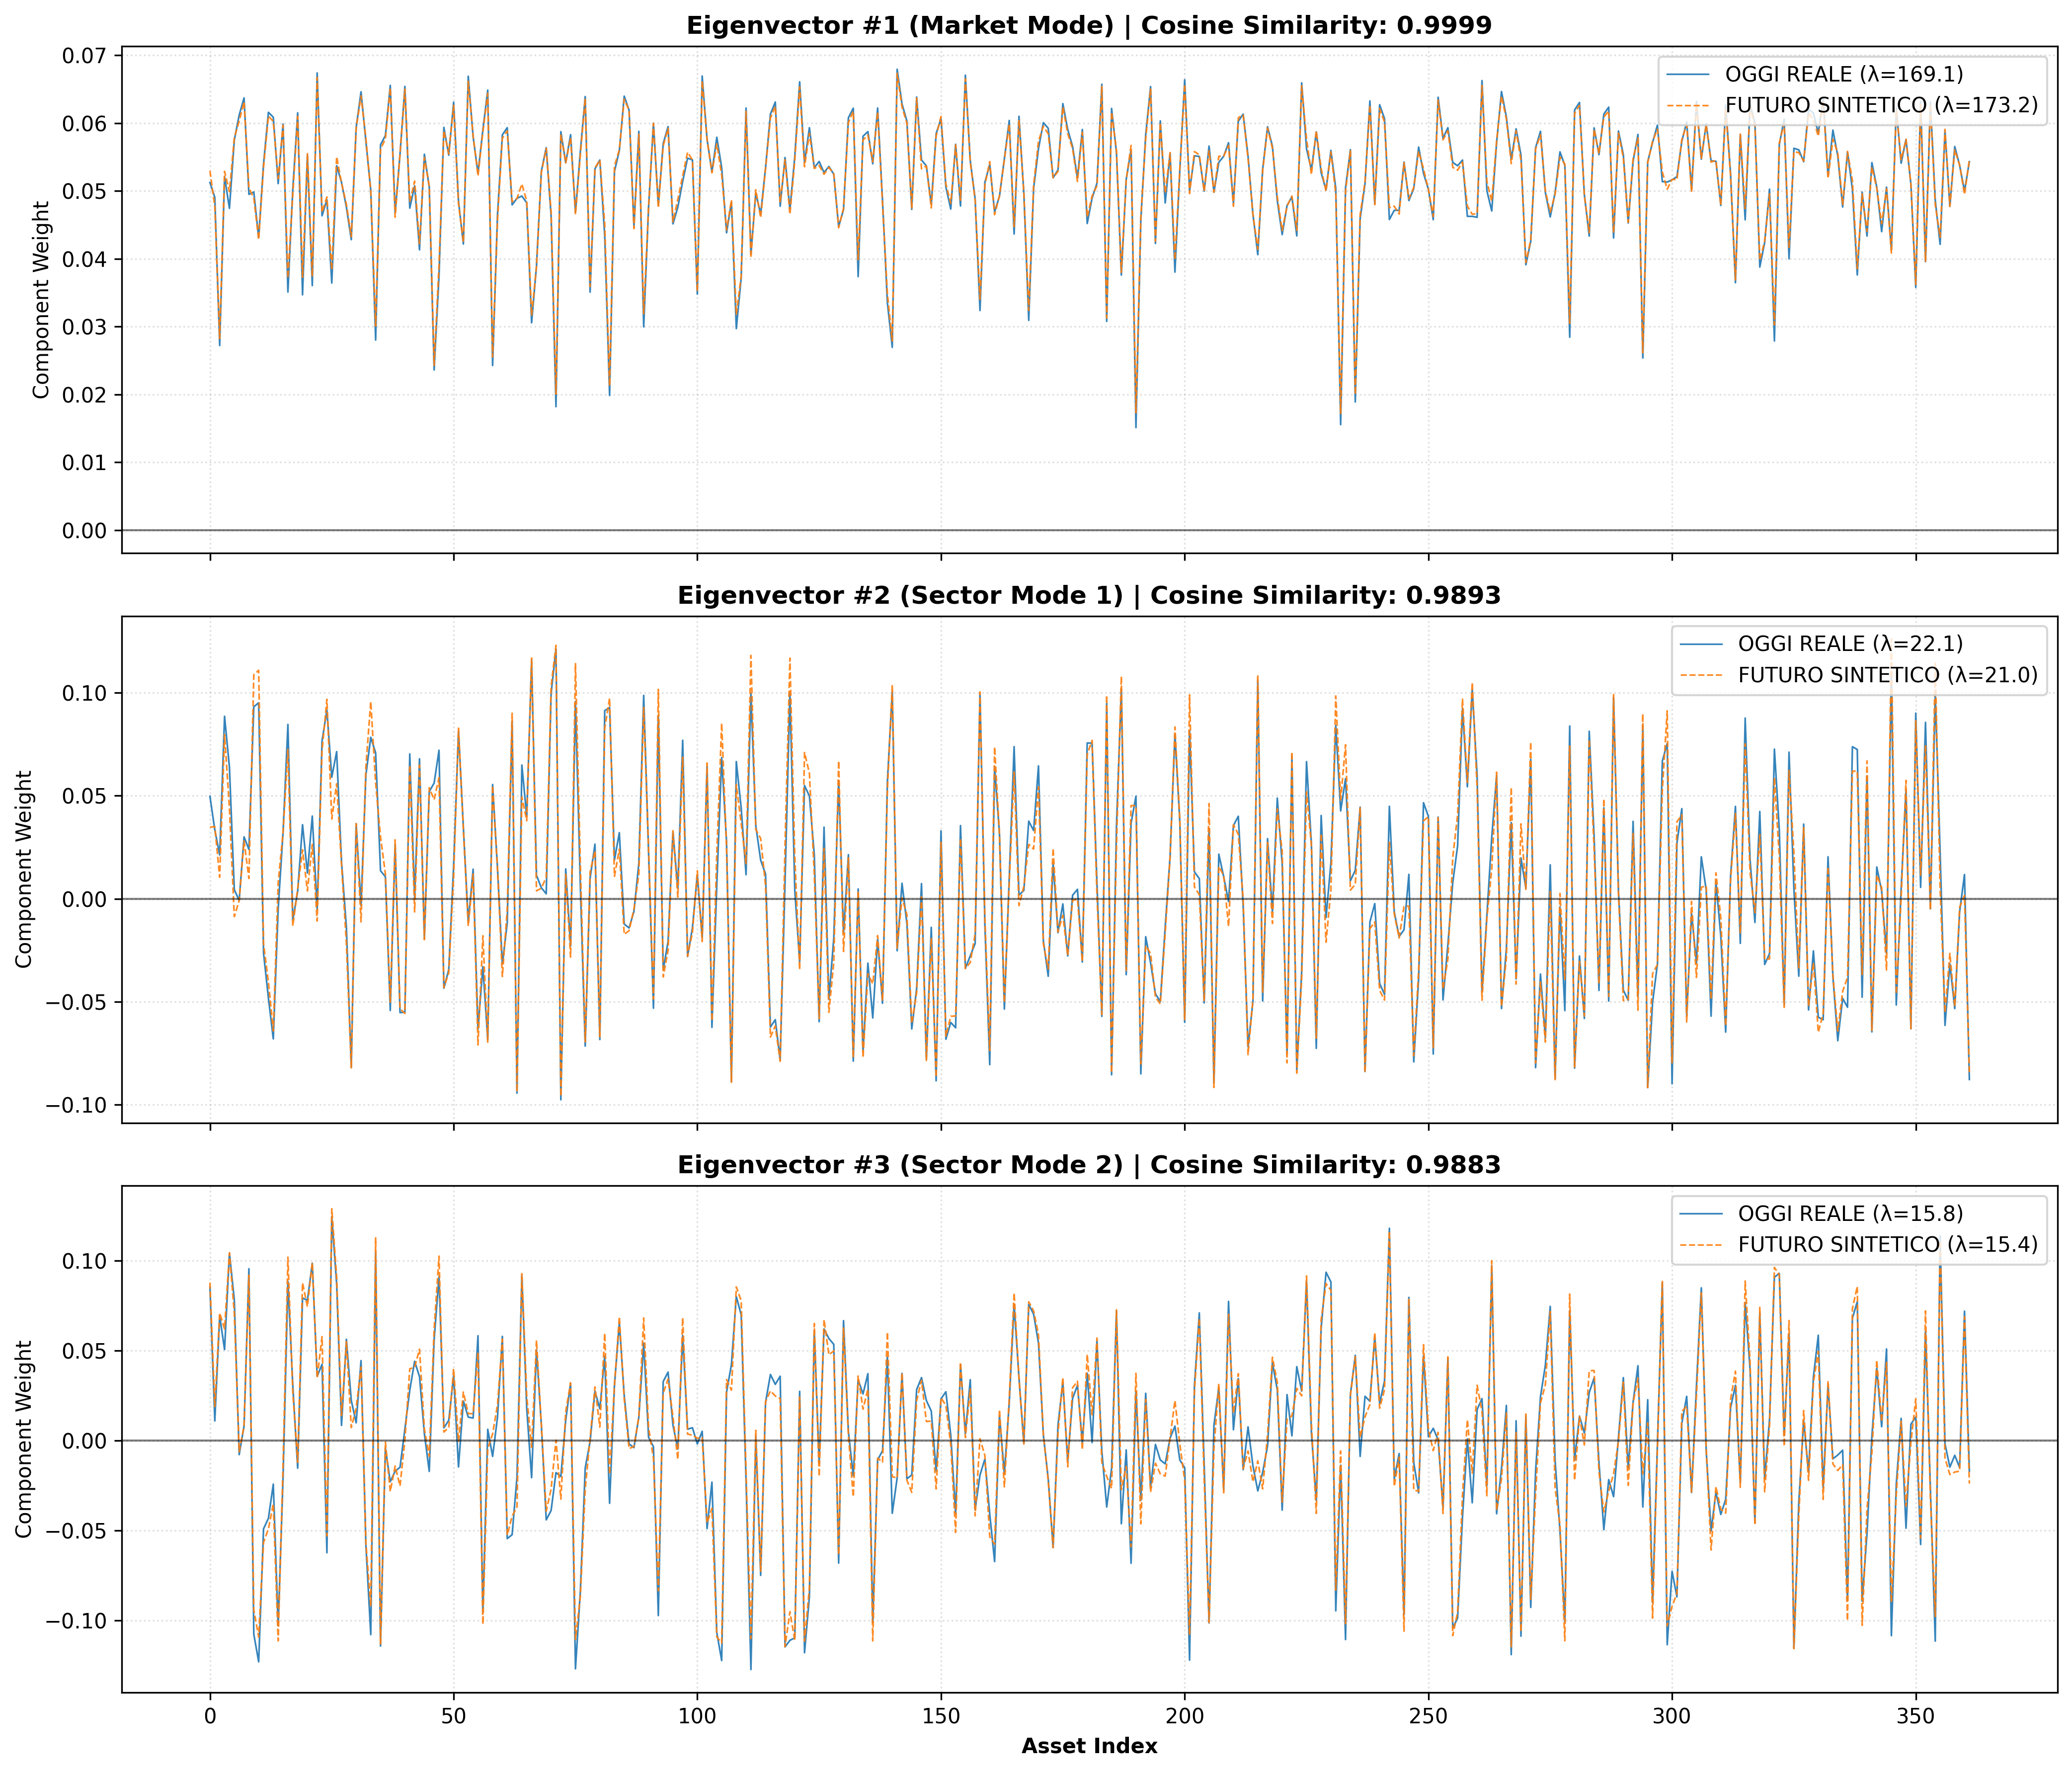
\includegraphics[width=0.85\textwidth]{./Pictures/capitolo8/fig_perron_frobenius_generato.png}
\caption{Confronto dei primi tre autovettori tra matrice odierna e matrice sintetica: le componenti del \emph{market mode} (in alto) sono tutte dello stesso segno in entrambe le matrici.}
\label{fig:pf_generato}
\end{figure}

\paragraph{Struttura gerarchica.} Il dendrogramma ottenuto per clustering gerarchico sulla matrice sintetica (Figura~\ref{fig:dendrogram_generato}) riproduce visivamente un'organizzazione a blocchi molto simile a quella della matrice odierna, con gli stessi principali raggruppamenti settoriali riconoscibili nella struttura ad albero.

\begin{figure}[h!]
\centering
\includegraphics[width=0.95\textwidth]{./Pictures/capitolo8/fig_dendrogram_generato.png}
\caption{Dendrogrammi comparativi per la matrice odierna (in alto) e la matrice sintetica a un mese (in basso).}
\label{fig:dendrogram_generato}
\end{figure}

\paragraph{Topologia scale-free del MST.} L'esponente della legge di potenza stimato sulla distribuzione di grado del Minimum Spanning Tree (Figura~\ref{fig:mst_generato}) risulta $\gamma_{\text{oggi}} = -2.119$ per la matrice odierna e $\gamma_{\text{futuro}} = -2.227$ per lo scenario sintetico: entrambi i valori confermano la natura \emph{scale-free} della topologia di rete, con un grado massimo di 15 e 14 connessioni rispettivamente.

\begin{figure}[h!]
\centering
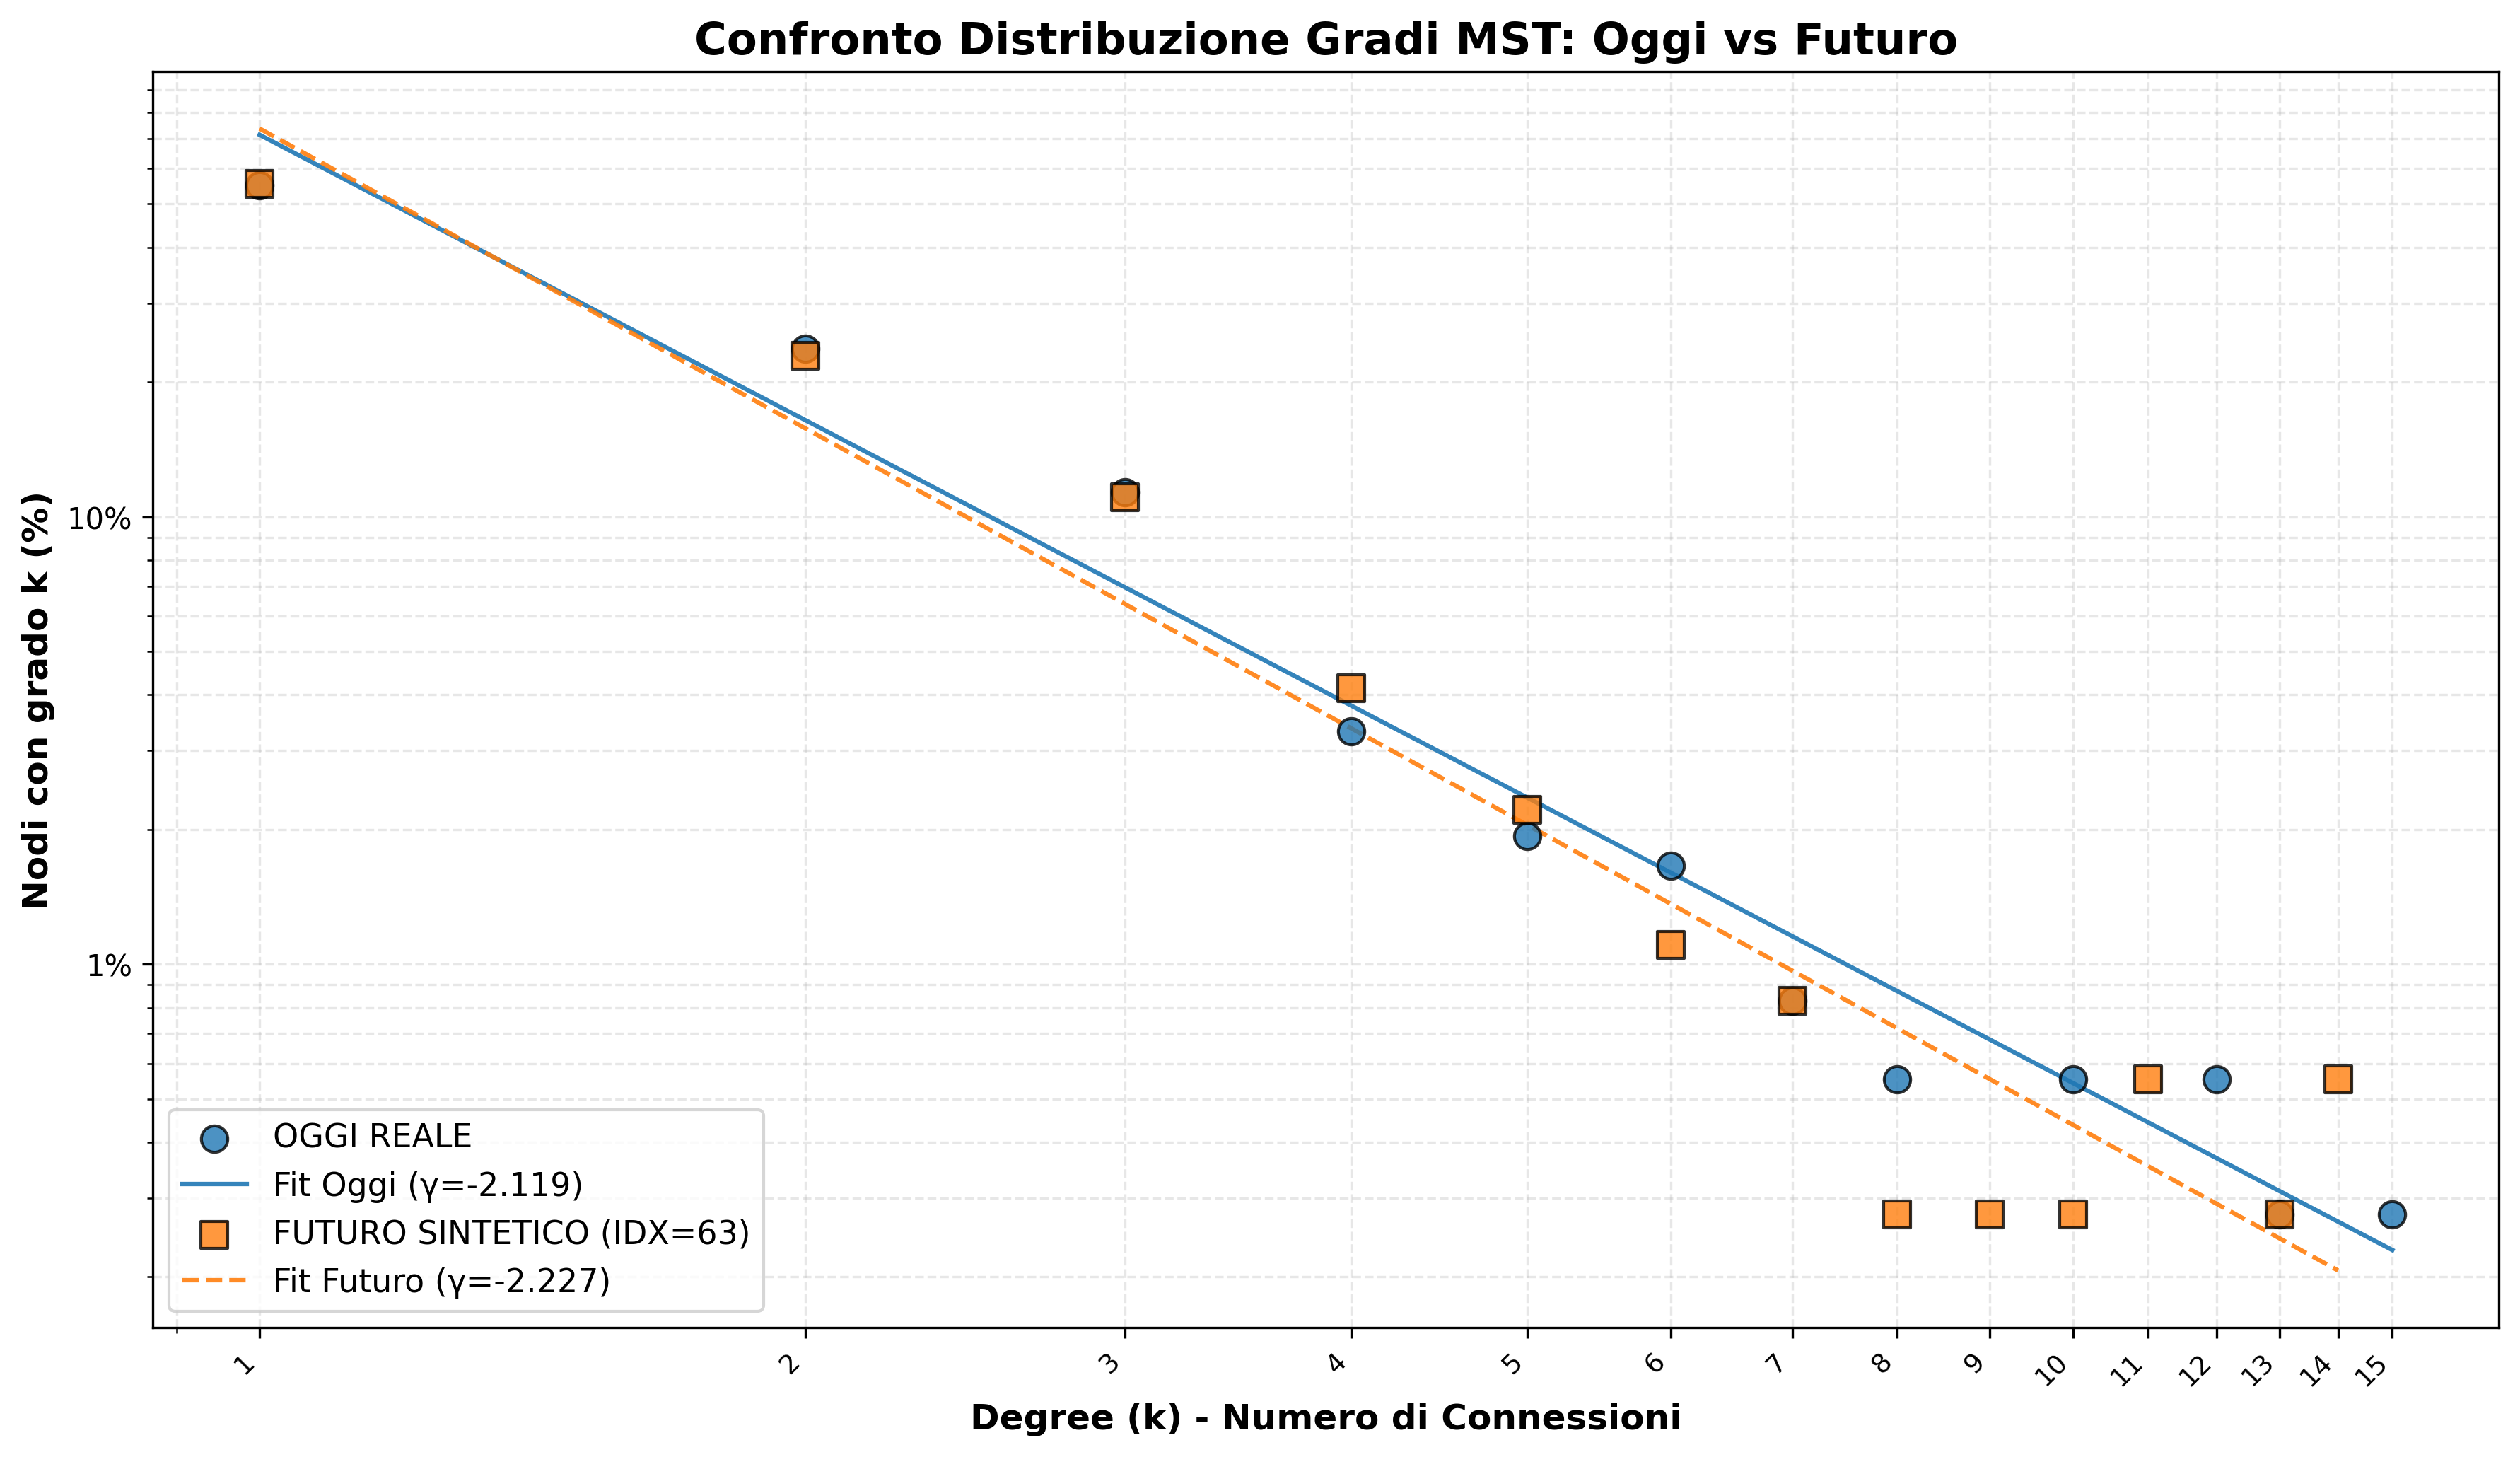
\includegraphics[width=0.75\textwidth]{./Pictures/capitolo8/fig_mst_degree_generato.png}
\caption{Distribuzione di grado del Minimum Spanning Tree in scala log-log, matrice odierna vs matrice sintetica a un mese.}
\label{fig:mst_generato}
\end{figure}

\section{Limiti della validazione e sviluppi futuri}
\label{sec:limiti_validazione}

\begin{osservazione}
La verifica presentata in questa sezione, pur non avendo evidenziato alcuna violazione dei cinque fatti stilizzati, è condotta \textbf{su un singolo scenario per volta} scelto tra i 1000 generati, e non in forma aggregata sull'intero insieme. Una validazione statisticamente più esaustiva richiederebbe di ripetere l'analisi (o quantomeno le metriche riassuntive: percentuale di scenari con proprietà di Perron-Frobenius soddisfatta, distribuzione dell'esponente $\gamma$, istogramma \emph{pooled} delle correlazioni \emph{pairwise}) sull'intero insieme di scenari generati, anziché su un singolo campione rappresentativo. Questo approfondimento è lasciato come sviluppo naturale del presente lavoro.
\end{osservazione}

Le matrici sintetiche generate in questo capitolo, avendo superato la verifica qualitativa sui cinque fatti stilizzati, costituiscono un insieme di scenari plausibili pronti per essere utilizzati come input di un motore di simulazione Monte Carlo per l'\emph{asset allocation} e la gestione del rischio di portafoglio (ad esempio per la stima del Value at Risk o dell'Expected Shortfall, sul modello di \citet{caprioli2024ptfvae}) --- applicazione che, per scelta di perimetro, non è stata affrontata in questo lavoro e viene proposta tra gli sviluppi futuri nelle Conclusioni.

% \input{./Part_III/capitolo9.tex}


%%%%%%%%%%%%%%%%%%%%%%%%%%%%%%%%%%%%%%%%%%%%%%%%
%%%%%%%%%%%%%%%%%%%%%%%%%%%%%%%%%%%%%%%%%%%%%%%%

%\bibliography{references}


\end{document}